\documentclass[headspline, 10pt, BCOR15mm, doubleside, ngerman, a5paper, DIV14]{scrbook}
%\documentclass[ebook,oneside,openany]{memoir}

\usepackage[ngerman]{babel}
\usepackage[utf8x]{inputenc}
\usepackage{graphicx}
\usepackage{longtable}
\usepackage[T1]{fontenc}
\usepackage{array}
\usepackage{pdfpages}
\usepackage[colorlinks,
    linkcolor=black,   % Farbe interner Verweise
    filecolor=black,   % Farbe externer Verweise
    citecolor=black]{hyperref}
\usepackage{marvosym} %% symbols (telephone, ..)
%%\usepackage[misc]{ifsym}

\let\Chaptermark\chaptermark
\def\chaptermark#1{\def\Chaptername{#1}\Chaptermark{#1}}
\let\Sectionmark\sectionmark
\def\sectionmark#1{\def\Sectionname{#1}\Sectionmark{#1}}
\let\Subsectionmark\subsectionmark
\def\subsectionmark#1{\def\Subsectionname{#1}\Subsectionmark{#1}}
\let\Subsubsectionmark\subsubsectionmark
\def\subsubsectionmark#1{\def\Subsubsectionname{#1}\Subsubsectionmark{#1}}

\newcommand{\tightlist}{}
%%\usepackage{amsmathamsfontsamssymb}


\begin{document}

\newcommand*{\includeimage}[1]{\includegraphics[width=1.0\textwidth]{#1}}
\newcommand*{\version}{1. Vorabversion}

\titlehead{}
\subject{}
\title{Informatik und Programmieren für Kinder}
\subtitle{Modulhandbuch für die Verwendung in Informatikkursen der Klassen drei bis sechs}
\author{Enactus~Aachen~e.~V.\and IT\emph{4}Kids}
\date{\today}
\publishers{Zusammengetragen und editiert von Steffen Schneider, Lucas Mosig, Dimitri Rusin und Leonhard Hetz}
\extratitle{\centering IT\emph{4}Kids Modulhandbuch \\ \copyright~2015~Enactus~Aachen~e.~V.\\\version}
\uppertitleback{\version~vom \today}
\lowertitleback{Dieses Material steht unter der Creative-Commons-Lizenz Namensnennung-Nicht kommerziell 4.0 International. Um eine Kopie dieser Lizenz zu sehen, besuchen Sie http://creativecommons.org/licenses/by-nc/4.0/.
\includegraphics[width=0.2\textwidth]{img/by-nc-eu.eps}}
\dedication{''I think everyone in this country should learn to program a computer. Everyone should learn a computer language because it teaches you how to think. I think of computer science as a liberal art.``\textit{-~Steve~Jobs}}
\maketitle


\frontmatter
\section*{Vorwort}
Informatik und Programmierung ist ein spannendes Fachgebiet, das eine hohe Bedeutung in unserem Alltag hat. Informatik und Programmierung ist überall gegenwärtig und wird ständig genutzt - dennoch ist das Angebot für informatische Bildung an Schulen in Deutschland oftmals kaum oder gar nicht vorhanden.

An vielen Schulen fehlen die Kapazitäten, sei es personell, sei es finanziell - dabei ist Informatik und Programmierung als spannendes Ergänzungsfach schon ab der dritten Klasse denkbar.

Ziel dieses Buchs soll sein, eine Basis für die Durchführung von Informatik-Kursen für Kinder im Grundschulalter und in der frühen Sekundarstufe~I zu bieten. Auf diese Weise können Sie als Lehrperson auch ohne tiefgreifende Informatikkenntnisse schnell Anregungen finden, wie Schülerinnen und Schüler an dieses spannende Feld herangeführt werden können.

Die Struktur des Buches ist bewusst offen gehalten und bietet eine Basis für einen sehr individuellen, auf Schülerinteressen angepassten Unterricht. Inhalt sind Projekte unterschiedlicher Themengebiete, die den Schülerinnen und Schülern auf vielfältige Weise die Grundkonzepte des Programmierens näher bringen. Mit steigender Lernkurve kann auch die Komplexität der Projekte schrittweise erhöht werden.

Das vorliegende Konzept wurde in einem einjährigen Modellversuch an einer Grundschule in Aachen im Jahr 2013/14 getestet und im Schuljahr 2014/15 an über zehn weiteren Schulen erfolgreich erprobt.

Unser Ziel ist es, Informatik flächendeckend an jeder Schule zu einem festen Bestandteil im Kursangebot zu machen. Die gewählten Projekte erfordern minimalen Einarbeitungsaufwand für Sie als Betreuerin oder Betreuer, werden aber zugleich alle denkbaren Schülerinteressen abdecken können. Überdies sind wir stets bemüht, die Inhalte des Modulhandbuchs weiter auszubauen.
\newpage
In diesem Sinne hoffe ich, dass dieses Werk Ihnen als Lehrperson eine Hilfe ist, einen spannenden Kurs vorzubereiten und den Schülerinnen und Schülern an Ihrer Schule die Möglichkeit zu bieten, einen erfolgreichen Einstieg in die Welt der Informatik zu finden.

\ \\Mit freundlichen Grüßen \\

\ \\Steffen Schneider\\
Aachen, den \today


\tableofcontents

\mainmatter
\chapter {Vorbereitung}

\section{Zu den Projekten}
Die Projekte gliedern sich in verschiedene Kategorien. Ziel ist es nicht, eine starre Unterrichtsstruktur vorzugeben. Aus bisheriger Erfahrung lässt sich sagen, dass die Auswahl der Materialien und Themen für den Kurs sehr entscheidend von der Kurszusammensetzung abhängt und dass eine korrekte Auswahl unabdingbar für das Gelingen des Kurses sein kann.

Aus diesem Grunde verfolgen wir in diesem Handbuch ein modulares Konzept: Die Projekte sind nicht allgemein nach Niveau (Anfänger, Fortgeschritten etc.) gegliedert, sondern in verschiedene Kompetenzbereiche unterteilt. Es gibt verschiedene Möglichkeiten, alle Bereiche abzudecken.

Trotz dieser bewusst offen gehaltenen Grundstruktur sollen an dieser Stelle einige beispielhafte Abläufe genannt werden, um die Kursplanung zu vereinfachen und einen schnellen Start zu ermöglichen.

\subsection{Kursvorschlag: Grundschule}

\begin{itemize}
	\item Einstieg: Labyrinth im Klassenraum %TODO link
    \item Erstes Projekt: Maus zum Käse
    \item Geschichten
    \item Klänge
    \item Aquarium
\end{itemize}

\subsection{Kursvorschlag: Weiterführende Schule}
\begin{itemize}
	\item Einstieg: Labyrinth im Klassenraum %TODO link
    \item Erstes Projekt: Labyrinth
    \item Einführungsprojekte
    \begin{itemize}
        \item Zeichnen und Farben
        \item Klänge
        \item Botschaften (zB Tanzstunde oder Bananen)
    \end{itemize}
    \item Wettrennen
    \item Pong
\end{itemize}


%TODO Schreiben

\section{Notwendige Tools}
Für die Durchführung der hier vorgestellten Projekte im Kurs kommen verschiedene Werkzeuge infrage, die im Folgenden vorgestellt werden sollen.

\subsection{Scratch Editor}
Scratch ist eine am MIT entwickelte, quelloffene Programmierumgebung. Scratch ist sowohl als Online- als auch als Offline-Version frei erhältlich.

es sowohl online als auch offline. Scratch ist die Standardumgebung, auf die für die Projekte in diesem Konzept zurückgegriffen wurde. Auf Scratch kann online unter \href{https://scratch.mit.edu}{scratch.mit.edu} zugegriffen werden.

\begin{figure}[ht]
	\centering
		\includeimage{img/Scratch}
	\caption[Scratch Online Editor]{Scratch Online Editor}
	\label{fig:scratch}
\end{figure}

Alle hier genannten Vorlagen mitsamt Beschreibungstext und Musterlösung sind online unter \href{http://www.it-for-kids.org/projects}{it-for-kids.org/projects} abrufbar. Zudem liegen die aktuellen Projektstände auf der mitgelieferten CD bereit.

Das Laden von Projekten in Scratch erfolgt durch Druck auf ''Entwickeln`` auf der Startseite. Wir empfehlen, im Kursbetrieb diese Seite als Lesezeichen oder Verknüpfung auf den Schülerrechnern zu hinterlegen.


\subsection{IT4Kids Online Editor}
Als Alternative zu Scratch sind wir bemüht eine eigene, auf die konkreten Bedürfnisse des Kursbetriebes zugeschnittene Entwicklungsumgebung anzubieten. Die Umgebung befindet sich derzeit in der aktiven Entwicklung und ist eine veränderte Version der ebenfalls quelloffenen Software \textit{Snap!}. Auf den IT4Kids Online Editor kann unter \href{http://code.it-for-kids.org}{code.it-for-kids.org} zugegriffen werden.

\subsection{IT4Kids Offline Editor}
Ebenfalls in der aktiven Entwicklung befindet sich der IT4Kids Offline Editor. Der aktuelle Entwicklungsstand kann auf unserer Homepage eingesehen werden.

\section{Vor Kursbeginn}

Vor Beginn eines IT4Kids Kurses empfehlen sich einige Vorkehrungen, die in diesem Abschnitt besprochen werden.

\subsection{Verfügbarkeit eines Beamers}
Bei vielen Projekten bietet es sich an, die fertigen Programme von den Schülerinnen und Schülern präsentieren zu lassen. Außerdem eignet sich ein Beamer sehr gut, um zu Beginn des Kurses das Stundenziel sowie das fertige Projekt zu zeigen. Sollte kein Beamer zur Verfügung stehen können Projekte an einem gut einsehbaren Rechner gezeigt werden. Manche Konzepte lassen sich auch gut an einer Tafel oder einem OHP demonstrieren.

\subsection{Infrastruktur zum Abspeichern von Projekten}
Zum Abspeichern von Projekten eignen sich grundsätzlich zwei Ansätze: Scratch unterstützt das manuelle Hoch- und Herunterladen von Projekten. Sofern an der Schule ein Netzwerkordner vorhanden ist, kann dieser für die Verteilung von Vorlagen und auch zum Abspeichern von Projekten verwendet werden.

Der zweite Ansatz ist eine Anmeldung auf der Scratch Homepage. Hier kann sich jede Schülerin und jeder Schüler einen eigenen Account zulegen. Einmal angemeldet, wird das jeweils aktuelle Projekt jeweils automatisch in der Cloud gespeichert.

In jedem Fall sollte im Vorfeld mit der Schule die Verfügbarkeit eines Netzwerkordners abgestimmt werden.

Auch die Verwendung von Schüler-USB-Sticks ist denkbar, sodass jeder Schüler seine Fortschritte für zuhause speichern kann. Es empfiehlt sich jedoch, die Projekte auch noch an einem anderen Ort zu speichern, da die SChüler ihre Sticks u.U. zuhause vergessen.

\subsection {Vor Stundenbeginn}
Als Kursbetreuer sollte vor dem Kurs das Projekt ausgewählt und verstanden werden. Dazu reicht es in der Regel sich das Lehrkonzept durchzulesen und die Programmierung in der Musterlösung nachzuvollziehen. Bei komplexeren Projekten kann es hilfreich sein sich bestimmte Programmteile zu notieren oder auf ein Cheat-sheet zurückzugreifen.
Erfahrungsgemäß ist es als Kursbetreuer ratsam sich deutlich vor Stundenbeginn im Kursraum einzufinden. So können die bisweilen etwas langsameren Schulrechner in aller Ruhe hochgefahren werden und auch Projekte und Scratchumgebung geöffnet werden. Dies kann andernfalls eine nicht unbeachtliche Zeit in Anspruch nehmen, was unter den Schülern zu Unruhe oder Unmut führt.

\chapter {Informatik mit Stift und Papier}

%Für den optimalen Einsatz dieses Lehrbuchs im Unterricht empfehle ich den Einsatz des Scratchsticks, der in diesem Kapitel unter anderem behandelt wird. Der Vorteil ist die Ausnutzung aller Unterrichtsmethoden, die den Schülerinnen und Schülern einen maximalen Lernerfolg bieten. Alternativ kann, wie oben schon beschrieben, auch auf den Scratch Editor (Version 1.4 offline, Version 2 online oder Version 2 Beta online) oder den Snap Editor (online und offline) zurückgegriffen werden.

In den ersten ein bis zwei Unterrichtsstunden sollte den Schülern, insbesondere wenn diese noch keinerlei Zugang zur Informatik hatten, kurz dargelegt werden, was Informatik eigentlich ist und mit welchen Mitteln im Unterricht gearbeitet wird. Dazu kann die Lehrperson kreativ werden oder aber auch eine Einführung aus diesem Buch verwenden.

\section{Zauberwürfel}\label{zauberwuxfcrfel}

Materialien: Ein Zauberwürfel(``Rubicks Cube'') Schwierigkeit: Eher für
ältere Schüler

Der Zauberwürfel sollte bis auf einige verbleibende Drehungen gelöst
sein, auf jeden Fall muss die Lösung relativ offensichtlich sein. Einem
Schüler werden die Augen verbunden, er erhält anschließend den Würfel,
den er vor sich auf den Tisch legt.

Anschließend haben die Kinder die Möglichkeit, nacheinander dem
Probanten Anweisungen zu geben. Dazu kann das vorliegende Spektrum an
``Befehlen'' genutzt werden:

\begin{itemize}
\item
  Drehe nach oben: Der Schüler dreht den Würfel so, dass die von ihm
  weg gerichtete Seite nun in Richtung Decke zeigt
\item
  Drehe nach rechts: Der Schüler dreht den Würfel so, dass die von ihm
  nach links ausgerichtete Seite nun in Richtung Decke zeigt
\item
  Verändere: Der Schüler dreht die obere ``Scheibe'' des Würfels im
  Uhrzeigersinn
\end{itemize}

Die Befehle sind bewusst auf ein Minimum reduziert, gerade so, dass das
Problem lösbar ist. Während dem Schüler die Befehle mitgeteilt werden,
schreibt die Lehrperson oder ein weiterer Schüler die Befehle an die
Tafel. Nach einiger Zeit sollte das Problem gelöst sein, wenn vielleicht
auch nicht optimal. Dann wird der Würfel an einen weiteren Schüler
gegeben (wieder entsprechend präpariert), der die Augenbinde erhält. Ein
weiterer Schüler liest das Programm vor, das anschließend umgesetzt
wird.

Optional ist es möglich, die Schüler mit der Frage zu konfrontieren, wie
der erste Zustand wiederhergestellt werden kann und wie sich das Problem
noch effizienter lösen lässt.

%// TODO lege als Tabelle an!

\section{Labyrinth}\label{labyrinth}

Wie Zauberwürfel, nur mit einem Labyrinth mit Stift und Papier.
Mögliches Szenario: Zuerst sieht man das Labyrinth auf eine
Übersichtskarte, anschließend allerdings nur noch einen schwarzen
Hintergrund, trotzdem muss man den Ausgang finden

\section{Labyrinth im Klassenraum}\label{labyrinth-im-klassenraum}

Ein Schüler erhält eine Augenbinde, im Klassenraum wird ein kleiner
Parcours aufgebaut. Die anderen Schüler müssen durch Anweisungen aus dem
untenstehenden Befehlssatz versuchen, den Schüler sicher und ohne
anzuecken durch den Klassenraum zu geleiten.

\begin{itemize}
\item
  Schritt vor
\item
  Drehe nach rechts (Drehung um 90 Grad nach rechts)
\item
  Drehe nach links (Drehung um 90 Grad nach links)
\end{itemize}

Dieses Experiment kann sehr gut als Einstieg genutzt werden, um die
Unterschiede in der ``Genauigkeit'' von realer Welt und Computer zu
verdeutlichen. Das Programm wird hier beim zweiten Schüler vermutlich
aufgrund anderer Schrittweiten o. ä. nur noch ansatzweise funktionieren.
Anschließend kann das Experiment ``Programmieren mit Stift und Papier''
gewissermaßen als Kontrast verwendet werden.

\section{Labyrinth mit Folie und
Papier}\label{labyrinth-mit-folie-und-papier}

Es ist teilweise in den Klassenzimmern nicht möglich die Tische zu
verrücken um ein Labyrinth zu bauen. Der Grund dafür ist entweder, dass
die Tische am Boden fest montiert sind oder Teilweise ist auch die
Gruppengröße für das Klassenraumprojekt nicht angemessen. In diesem Fall
gibt es die Alternative für eine Übung in Kleingruppen am Arbeitsplatz.
Man dasselbe Experiment auch mit einem augedruckten Labyrinth in kleinen
Gruppen durchgeführt werde. Man bildet kleine Gruppen bis zu einer
Gruppengröße von bestelnfalls 3 bis maximal 5 Personen. Jede Gruppe
erhält eine Folie, ein Papier mit einem Raster und ein Papier, auf dem
das Labyrinth abgedruckt ist. Eine Person in der Gruppe darf das
Labyrinth sehen und der Zeichnenden Person anweisungen geben. Ein
Gruppenmitglied ist der Zeichner. Dieses Gruppenmitglied hat die Aufgabe
auf der Folie , die auf dem Rasterpapier liegt, die Anweisungen der
Person aufzuzeichnen, die das Labyrinth lösen muss. Eine dritte Person
schreibt die Befehle untereinander auf, die die Anweisende Person gibt.
So entsteht ein Programm.

Der Befehlssatz besteht hier aus:

\begin{itemize}
\item
  Ein Kästchen vor
\item
  Drehe links (um 90 Grad)
\item
  Drehe rechts (um 90 Grad)
\end{itemize}

Im Anschluss an diese Übung kann dasselbe Labyrinth mit Scratch gelöst
werden. Hier kann in Anlehnung an das in der Gruppe erstellte Programm
eine Maus durch das Labyrinth zum Käse geführt werden. Dieses Projekt
vereint das Projekt ``Maus zum Käse'' und ``Labyrinth''. Für Schüler,
die bereits sehr schnell das erste Programm in Scratch fertiggestellt
haben, liegt im Anhang ein anspruchsvolleres Labyrinth vor, um das
Erlernte zu vertiefen.

Die Parallelen zur allgemeinen Programmierung können mit diesem Projekt
sehr schön bildhaft dargestellt werden. Die Kinder sollen verstehen, wie
der Programmierer mit dem Computer und der Entwicklungsumgebung
arbeitet. Dafür werden zu Beginn drei Rollen verteilt:

\begin{itemize}
\item
  \emph{Programmierer} : Anweisende Person, dieser erhält das Labyrinth
  auf Folie. Der Programmierer kennt damit das zu lösende Problem, kann
  es aber nur mithilfe des Computers lösen
\item
  \emph{Computer}: Der ``Computer'' erhält ein leeres Blatt Papier mit
  einem vorgezeichneten Raster. Auf dieses wird Schritt für Schritt der
  Weg eingezeichnet, den der Programmierer vorsagt. Der Computer hat
  also keine Kenntnis über das Problem und befolgt lediglich die
  Anweisungen des Programmierers.
\item
  \emph{Entwicklungsumgebung/Sekretär}: Damit der Programmierer das
  Problem lösen kann, ohne bei jedem Durchlauf die Befehle neu zu
  überlegen, werden alle Anweisungen auf einem leeren Blatt Papier
  festgehalten. Wenn das Problem dann einmal fertig gelöst ist, kann mit
  diesen Anweisungen das Labyrinth immer wieder durchlaufen werden.
\end{itemize}

\subsection{Erweiterungen}\label{erweiterungen}

Wenn das Problem mit einfachen Anweisungen gelöst ist, kann als neuer
Befehl die ``Wiederhole''-Struktur eingeführt werden. Mit dem Befehl

Wiederhole (N Mal)

wird der darauffolgenden Befehl entsprechend wiederholt ausgeführt. Die
Schülerinnen und Schüler können dann mit diesem neuen Befehl ihr
Programm entsprechend vereinfachen.

Mit leichten Abstrichen lässt sich diese Vorgehensweise, wenn nötig,
auch auf einer Tafel durchführen.

\subsection{Überleitung}\label{uxfcberleitung}

Nach erfolgreichem Abschluss des Projekts kann die Arbeit am PC
beginnen. Empfohlenes Projekt für den Anschluss ist wahlweise ``Maus zum
Käse'' vor allem für jüngere Schülerinnen und Schüler aus der
Grundschule oder auch ``Labyrinth''.

\chapter {Projekte zum Einstieg}

In diesem Kapitel werden Projekte für den einfachen Einstieg in Scratch und damit die Programmierung im Allgemeinen behandelt. Sie sind in der Regel, je nach Gruppe, im Rahmen einer Unterrichtsstunde umsetzbar.
Die meisten Einstiegsprojekte sind so konzipiert, dass sie eine relativ spezifische Fähigkeit vermitteln sollen, weshalb sie teilweise auch später noch hilfreich sein können.

\section{Bananen hergezaubert}\label{bananen-hergezaubert}

\textbf{Erforderliche Kompetenzen:}\\
Bewegung

\textbf{Gewonnene Kompetenzen:}\\
Klone, Senden und Empfangen, Zufall

\begin{figure}[ht]
    \centering 
    \includeimage{img/23.png}
    \caption[\Sectionname]{\Sectionname}
\end{figure}

\subsection{Beschreibung}\label{beschreibung}

Der Zauberer oben links wird mehrmals angeklickt, woraufhin er aus einer
Banane sehr, sehr viele herzaubert. Dieses Projekt bietet eine
Möglichkeit Zufall und Botschaften (in diesem Fall als ``Zauber'')
anschaulich zu machen

\subsection{Durchführung}\label{durchfuxfchrung}

\subsubsection{Phase 1: Planung}\label{phase-1-planung}

In der Planungsphase werden mit den Schülern die folgenden Dinge
besprochen:

\begin{itemize}
\item
  Wie klont man eine Figur? Wie steuert man den Klon? Was bedeuten die
  Klonbefehle unter ``Steuerung''?
\item
  Wie bewegt sich der Klon? Wie wählt er sein Ziel aus?
\item
  Was ist der Trigger für das Klonen? Welche Rolle spielt dabei der
  Zauberer?
\end{itemize}

\subsubsection{Phase 2: Vorbereitungen}\label{phase-2-vorbereitungen}

In der Vorbereitungsphase suchen sich die Schüler die Figuren aus:
Zauberer, Zauberteppich, Banane und Affe. Selbstverständlich können auch
diverse andere Kombinationen aus den verfügbaren Figuren der
Scratch-Spritebibliothek verwendet oder Schüler können sich selbst etwas
malen.

\subsubsection{Phase 3: Programmierung}\label{phase-3-programmierung}

\begin{enumerate}
\item
  Die Banane klont sich selbst
\item
  Der Klon gleitet an eine zufällig gewählte Spielfeldposition
\item
  Die Banane klont sich selbst genau dann, wenn der Zauberer angeklickt
  wird
\item
  Optional können verschiedene Geräusche und Farbeffekte an den
  passenden Stellen eingebaut werden
\end{enumerate}

\subsubsection{Detaillierte
Programmbeschreibung}\label{detaillierte-programmbeschreibung}

Die Musterlösung funktioniert folgendermaßen: Bananen erzeugt einen Klon
von sich selbst, wenn sie die Nachricht ``Teilt euch!'' erhält. Im
``When I start as a clone''-Block gleitet Bananen in zufällig bestimmt 1
bis 10 Sekunden zu einer ebenfalls zufällig gewählten Spielfeldposition.
Zauberer versendet die Nachricht ``Teilt euch!'' in dem Moment, das sie
angeklickt wird.

\subsubsection{Phase 4: Testen und
vorstellen}\label{phase-4-testen-und-vorstellen}

In der Vorstellungsphase kann ein beliebiger Schüler sein Spiel
vorstellen, falls er es möchte. Dabei kann man explizit auf die
einzelnen Teilprobleme hinweisen, welche der Schüler gelöst hat. Aber
man kann die anderen auch fragen, was er verbessern könnte, wenn er an
diesem Projekt nächste Stunde noch arbeiten will.

\subsection{Erweiterungen}\label{erweiterungen}

Es wäre denkbar, dass der Affe mit den Pfeiltasten bewegt werden kann
und dabei die berührten Bananen gegessen werden.

\section{Maus zum Käse}\label{maus-zum-kuxe4se}

\textbf{Erforderliche Kompetenzen:}\\
keine

\textbf{Gewonnene Kompetenzen:}\\
BEWEGUNGEN

\begin{figure}[ht]
    \centering 
    \includeimage{img/29.png}
    \caption[\Sectionname]{\Sectionname}
\end{figure}

\subsection{Beschreibung}\label{beschreibung}

Dieses Projekt kann relativ gut skaliert werden, von einem recht
einfachen bis zu einem recht umfangreichen Schwierigkeitsgrad. Primäres
Ziel ist die Einführung von \emph{Bewegungen} und erste Erfahrung mit
den Funktionen aus der Kategorie \emph{Fühlen}. Optional kann auch mit
den grundlegenden Funktionen aus der Kategorie \emph{Steuerung}
gearbeitet werden.

Das Projekt enstand als Anlehnung an die manuell durchgeführten
Labyrinth Versuche. Als Spielfiguren kommen eine Maus und ein Stück Käse
zum Einsatz. Die Maus befindet sich auf einer Insel, die über einen
Holzsteg mit einer anderen Insel verbunden ist. Die Schülerinnen und
Schüler sollen nun versuchen, mithilfe von hintereinander ausgeführten
Bewegungen die Maus bis zum Käse zu bringen. Im ersten Anlauf können die
einzelnen Befehle dabei manuell angeklickt werden, wenn alles
funktioniert, wird alles zu einem Programm zusammengefasst.

\subsection{Erweiterung}\label{erweiterung}

Schnelle Schüler können versuchen, die Maus auf Tastendruck reagieren zu
lassen und sie somit zu steuern. Zudem können mehrere ``Level'' gespielt
werden, indem weitere Hintergrundbilder angelegt werden.

\section{Labyrinth}\label{labyrinth}

\textbf{Erforderliche Kompetenzen:}\\
keine

\textbf{Gewonnene Kompetenzen:}\\
Scratch-Umgebung kennen lernen

Ereignisse \{Startbedingung (Wenn angeklickt)\}

Bewegung \{Koordinaten (gehe, gehe in zu), Winkel (drehe dich)\}

Steuerung \{Wiederholungen (wiederhole)\}

\begin{figure}[ht]
    \centering 
    \includeimage{img/30.png}
    \caption[\Sectionname]{\Sectionname}
\end{figure}

\subsection{Beschreibung}\label{beschreibung}

Mit dem Start des Programms soll die Maus ohne weitere Eingabe das
Labyrinth bis zum Ziel durchlaufen.\\
Bei der Schlüsselvariante muss die Maus vorher auf den Schlüssel
navigieren, damit sich das Tor öffnet.

\subsection{Durchführung}\label{durchfuxfchrung}

\subsubsection{Phase 1: Planung}\label{phase-1-planung}

In der Planungsphase werden mit den Schülern die folgenden Punkte
besprochen:

\begin{itemize}
\tightlist
\item
  Wie und wodurch wird ein Programmteil gestartet? Welchen Einfluss hat
  dies auf andere Programmteile?
\item
  Wie Programmiere ich eine spezielle Figur und nicht versehentlich eine
  andere?
\item
  Was sind Koordinaten und Winkel? Wie kann ich diese ablesen? (Dieser
  Punkt ist optional, gerade in der Grundschule kann das Verständnis von
  Gradzahlen/Winkeln und Koordinaten auf einen späteren Zeitpunkt mit
  einem spezifischen Projekt verschoben werden.)
\end{itemize}

\subsubsection{Phase 2: Vorbereitungen}\label{phase-2-vorbereitungen}

Hierbei ist eine Einarbeitung vorgesehen: Wo bearbeitet man die Figuren,
Info der Figuren, Koordinaten und Winkel ablesen, Wo sind die Skripte
gehe, drehe dich, \ldots{} zu finden.

\subsubsection{Phase 3: Programmierung}\label{phase-3-programmierung}

Die verwendeten Befehle sind:

\begin{itemize}
\tightlist
\item
  wiederhole \ldots{} mal
\item
  gehe \ldots{} er-Schritt
\item
  drehe dich um \ldots{} Grad
\item
  Diese Schritte müssen so oft wiederholt werden, bis die Maus das Ziel
  erreicht hat.
\end{itemize}

\subsubsection{Phase 4: Testen und
vorstellen}\label{phase-4-testen-und-vorstellen}

In der Vorstellungsphase können die Schüler ihre Lösung vorstellen,
wodurch die unterschiedlichen Arten der Lösung erläutert werden können.
Dabei sollte jedoch der spielerische Spaß im Vordergrund stehen und
nicht abschreckend wirken.

\subsection{Erweiterungen}\label{erweiterungen}

Als Erweiterung zum Labyrinth steht noch Labyrinth mit Schlüssel zur
Verfügung, in diesem Können sie sich weiter mit der Problematik
auseinander setzen und eine andere Variation der
Programmiermöglichkeiten aneignen.

\section{Buchstaben}\label{buchstaben}

\textbf{Erforderliche Kompetenzen:} Scratch-Umgebung kennen

\textbf{Gewonnene Kompetenzen:}\\
Figuren auswählen/bearbeiten, Ereignisse, Bewegung (gehe zu, drehe
dich), Steuerung \{Wiederholungen (wiederhole)\}

\begin{figure}[ht]
    \centering 
    \includeimage{img/32.png}
    \caption[\Sectionname]{\Sectionname}
\end{figure}

\subsection{Beschreibung}\label{beschreibung}

Es soll ein Programm erstellet werden, in welchen beliebige Figuren
(beisielsweise Buchstaben) wackelnd, drehend, größer oder kleiner
werdend, \ldots{} zu einer sinnvollen Endposition (einem Wort) gleiten.

\subsection{Durchführung}\label{durchfuxfchrung}

In der Planungsphase werden mit den Schülern die folgenden Punkte
besprochen:

\subsubsection{Phase 1: Planung}\label{phase-1-planung}

\begin{itemize}
\tightlist
\item
  Welche Möglichkeiten stehen mit bei den Figuren zur Verfügung? Wie
  wähle ich diese aus?
\item
  Wie Programmiere ich eine spezielle Figur und nicht versehentlich eine
  andere?
\item
  Was sind Koordinaten und Winkel? Wie kann ich diese ablesen?
\end{itemize}

\subsubsection{Phase 2: Vorbereitungen}\label{phase-2-vorbereitungen}

In der Vorbereitungsphase suchen sich die Schüler die Figuren aus. Diese
können sie auch noch beliebig bearbeiten und ihrer Kreativität freien
Lauf lassen indem sie z.B. auch weitere Figuren selber malen.

\subsubsection{Phase 3: Programmierung}\label{phase-3-programmierung}

Die nötigen Schritte sind:

\begin{itemize}
\tightlist
\item
  Beim Start Figuren zum Chaospunkt Position springen lassen.
\item
  Figuren drehend, \ldots{} zum geordneten Position bewegen.
\end{itemize}

\subsubsection{Phase 4: Testen und
vorstellen}\label{phase-4-testen-und-vorstellen}

In der Vorstellungsphase können die Schüler ihre eigenständig
Programmierten Spiele vorstellen, um den anderen Ihre Kreativität zu
zeigen und den anderen dadurch weitere Anregungen für die nächste Stunde
zu geben.

\subsection{Erweiterungen}\label{erweiterungen}

Als Erweiterung zu Buchstaben besteht die Möglichkeit den Schülern das
Projekt mit Musik hinterlegen zu lassen, oder die Figuren mit kleinen
Änderungen mehrmals einfügen, um diese dann geschickt wechselnd eine
Bewegung Simulieren zu lassen oder einfach nur die Farbe ändernd.

\section{Farben}\label{farben}

\textbf{Erforderliche Kompetenzen:} keine

\textbf{Erworbene Kompetenzen:} Fühlen, Bedingungen

\begin{figure}[ht]
    \centering 
    \includeimage{img/33.png}
    \caption[\Sectionname]{\Sectionname}
\end{figure}

\subsection{Beschreibung}\label{beschreibung}

Bei diesem Projekt geht es darum, die verschiedenen Funktionen aus der
Klasse \emph{Fühlen} zu testen. Grundsätzlich bekommen die Schülerinnen
und Schüler einen zwei- oder mehrfarbigen Hintergrund. Auf Basis der
Hintergrundfarbe soll sich das Aussehen der Figur verändern. Dabei kann
die Figur zwischen den einzelnen Bereichen verschoben werden.

In einer Endlosschleife soll immer die aktuelle Hintergrundfarbe
abgefragt werden. Dies geschieht über die entsprechende Funktion in der
Befehlsgruppe ``Fühlen''. Über eine Falls-Bedingung kann abgefragt
werden, ob die Hintergrundfarbe der gewählten entspricht. Ist dies der
Fall, so soll eine bestimmte Aktion ausgeführt werden. Obligatorisch
wäre eine Ausgabe in einer Sprechblase, hier kann den Schülern aber
grundsätzlich Freiraum für eigene Experimente gelassen werden.

\subsection{Vorbereitung}\label{vorbereitung}

Sehr wichtig für die Durchführung dieses Projekts ist die Einführung von
Kontrollstrukturen. Das Programm später wird auf die ``Falls \ldots{}
Dann'' Abfrage zurückgreifen, diese sollte also in der Vorbereitung
vorab angesprochen werden.

Der entsprechende Block findet sich in der Kategorie ``Steuerung''. Als
Argument muss in den Block noch ein weiterer Befehl eingesetzt werden.
Im Falle dieses Projekts handelt es sich dabei um einen Block aus der
Kategorie ``Fühlen''. Hier stehen zahlreiche Funktionen bereit, so wie
die Kollisionserkennung mit anderen Objekten, dem Mauszeiger oder dem
Rand auch das Abfragen der Hintergrundfarbe, was wir uns in diesem
Projekt zunutze machen wollen.

In der Vorbereitung sollte den Schülerinnen und Schülern nun vermittelt
werden, dass mithilfe dieser Kontrollstrukturen eine Abfrage der
Hintergrundfarbe mit anschließendem Ausführen einer Aktion möglich ist.

\subsection{Programmierung}\label{programmierung}

Die erste Aufgabe ist es, die Hintergrundfarbe als Text auf dem
Bildschirm auszugeben. Dazu kann der entsprechende Befehl aus der Klasse
``Aussehen'' verwendet werden.

In der Vorlage steht ein Hintergrund mit verschiedenen Farben bereit.

Die Programmabfolge soll nun so aussehen, dass die Figur mit der Maus
auf eine Farbe gezogen wird. Sobald die Figur angeklickt wird, soll die
aktuelle Farbe ausgegeben werden.

Zur Lösung ist die Verwendung einer Kontrollstruktur pro Farbe notwenig,
gekoppelt an die jeweilige Ausgabe der Farbe.

\subsection{Erweiterungen}\label{erweiterungen}

Für dieses Projekt sind einige Änderungen denkbar: Schülerinnen und
Schüler zeichnen den Hintergrund selbst, statt die Vorlage zu
verwenden.\\
Nach Fühlen einer anderen Farbe ist eine Kostümänderung anstelle einer
Ausgabe in einer Sprechblase denkbar.

\section{Tanzstunde}\label{tanzstunde}

Erforderliche Kompetenzen: Scratch-Umgebung kennen\\
Gewonnene Kompetenzen: Startbedingungen, Nachrichten, Wiederholungen,
Kostüme, Klänge/Instrumente

\begin{figure}[ht]
    \centering 
    \includeimage{img/36.png}
    \caption[\Sectionname]{\Sectionname}
\end{figure}

\subsection{Beschreibung}\label{beschreibung}

Wird die oberste Figur, der Tanzlehrer, angeklickt, sendet er eine
Nachricht an alle Tänzer, das sind die anderen drei Figuren unter ihm.
Beim empfangen dieser Nachricht beginnen die Tänzer, zu tanzen, und
Musik zu machen. Die Tänzer tanzen, indem sie ihre Kostüme wechseln.

\subsection{Durchführung}\label{durchfuxfchrung}

\subsubsection{Phase 1: Planung}\label{phase-1-planung}

In der Planungsphase werden mit den Schülern die folgenden Punkte
besprochen:

\begin{itemize}
\item
  Wie wird eine Nachricht (``Message'') versandt und empfangen
\item
  Wie werden einer Figur mehrere Kostüme zugewiesen und diese im
  Programm geändert
\item
  Welche Möglichkeiten gibt es, Klänge zu erzeugen
\end{itemize}

\subsubsection{Phase 2: Vorbereitung}\label{phase-2-vorbereitung}

In der Vorbereitungsphase erstellen die Schüler die nötigen Figuren.
Diese können auch noch beliebig bearbeitet und kreativ veränder werden,
in z.Bsp.: weitere Kostüme hinzugefügt oder Figuren selber gemalt
werden.

Eine oder mehrere Bühnenbilder sind auch denkbar, welche dann zusätzlich
mit der Musik variieren können.

\subsubsection{Phase 3: Programmierung}\label{phase-3-programmierung}

\begin{itemize}
\item
  sende / empfange Message
\item
  nächstes Kostüm
\item
  warte \ldots{} Sek.
\item
  diese letzten beiden Schritte werden fortlaufend wiederholt
\item
  zwischen den Wiederholungen kann noch mit Klang gearbeitet werden
\end{itemize}

\subsubsection{Phase 4: Testen und
vorstellen}\label{phase-4-testen-und-vorstellen}

In der Vorstellungsphase können die Schüler ihre eigenständig
Individuellen Kreationen vorstellen. Dabei haben die Schüler die
Möglichkeit sich gegenseitig zu inspirieren.

\subsection{Erweiterungen}\label{erweiterungen}

Als Erweiterung dazu können die Schüler noch unter Daten eine Variable
hinzufügen, die die Anzahl der Klicks vom Tänzer zählt.

\section{Zeichnen}\label{zeichnen}

Erforderliche Kompetenzen: Bewegen\\
Gewonne Kompetenzen: Zeichnen, Bedingungen

Ziel des Projekts ``Zeichnen'' ist das tiefere Verständnis des
Koordiatensystems sowie der Drehwinkel. Außerdem werden Möglichkeiten
aufgezeigt, wie Formen auf den Bildschirm gezeichnet werden können.

\begin{figure}[ht]
    \centering 
    \includeimage{img/37.png}
    \caption[\Sectionname]{\Sectionname}
\end{figure}

\subsection{Vorbereitung}\label{vorbereitung}

Das Projekt sollte mit einer Einführung und einem anschaulichen Beispiel
an der Tafel begonnen werden. Dabei wird eine Schülerin oder ein Schüler
zur Tafel gebeten, um ein Quadrat zu zeichnen.

Dabei darf die Person an der Tafel nur den Anweisungen seiner
Mitschülerinnen und Mitschüler folgen. Aufgabe ist es, mittels der
Befehle

\begin{itemize}
\item
  Vorwärts
\item
  Drehe dich (wie weit?)
\end{itemize}

verschiedene Formen zu zeichnen. Für den Beginn eigenen sich Quadrate,
Dreiecke, Sechsecke und später auch ein Kreis.

Ziel des Projekts ist es, dass die Schülerinnen und Schüler mit den
verschiedenen Drehwinkeln vertraut gemacht werden. Mögliche Anweisungen
könnten dann etwa so aussehen:

\begin{itemize}
\item
  Quadrat: ``Vorwärts, Drehen (90 Grad), Vorwärts, Drehen (90 Grad),
  Vorwärts, Drehen (90 Grad), Vorwärts, Drehen (90 Grad)
\item
  Sechseck: Vorwärts, Drehen (60 Grad), Vorwärts, \ldots{}
\item
  Kreis: ein Stück vorwärts, Drehen, ein Stück vorwärts, \ldots{}
\end{itemize}

Diese Anweisungen können natürlich auch hier wie bei ``Informatik mit
Stift und Papier'' durch entsprechende \emph{Wiederhole}-Anweisungen
stark abgekürzt werden.

Welche Formen genau eingeführt werden, bleibt generell dem Kursbetreuuer
überlassen. Der Kreis ist als schwierigste Form anzusehen und kann auch
optional als ``Bonusaufgabe'' beim nun folgenden Programmieren für
besonders schnelle Schüler herangezogen werden.

\subsection{Zum Projekt}\label{zum-projekt}

Nach der Einführung sollten alle Schülerinnen und Schüler die Grundidee
des Projekts erfasst haben. Ziel ist es nun, die zuvor an der Tafel
gezeichneten Formen im Programm umzusetzen. Die Tafel mit dem
entsprechenden Anschrieb kann dabei je nach Stärke der Gruppe
verdeckt/zugeklappt werden oder aber auch offen bleiben und als Vorlage
dienen.

Die Aufgabe am PC ist, mit der Programmierumgebung mindestens drei
verschiedene Formen zu zeichnen.

\subsubsection{\texorpdfstring{Blöcke in der Gruppe
``Zeichnen''}{Blöcke in der Gruppe Zeichnen}}\label{bluxf6cke-in-der-gruppe-zeichnen}

In der Kategorie ``Zeichnen'' sind in der Programmierung alle wichtigen
Befehle zusammengefasst, die den sog. Malstift steuern. Dieser virtuelle
Stift greift im Mittelpunkt der jeweiligen Figur an und kann abgesetzt
und aufgenommen werden. Wenn der Stift abgesetzt ist, zieht die Figur
bei ihren Bewegungen eine Linie hinter sich her. Diese Linie soll hier
genutzt werden, um die Formen zu zeichnen.

\subsubsection{\texorpdfstring{Blöcke in den Gruppen ``Steuerung'' und
``Bewegung''}{Blöcke in den Gruppen Steuerung und Bewegung}}\label{bluxf6cke-in-den-gruppen-steuerung-und-bewegung}

Mit den Blöcken ``gehe (10)er Schritt'' und ``drehe dich um (15) Grad''
werden die Bewegungen realisiert. Zu beginn können mehrere dieser Blöcke
aneinandergereiht werden. Wenn die Schüler schnell zurecht kommen, kann
das Programm gekürzt werden, indem mehrere dieser Blöcke über die
Steuerungsblöcke ``wiederhole (10) mal'' zusammengefasst werden.\\
Die Geschwindigkeit der Bewegung kann über die Variation von
Wiederholungen und Schritten eingestellt werden.\\
Beispielsweise führen folgende Möglichkeiten zu der gleichen Strecke,
bei der ersten Möglichkeit bewegt sich die Figur aber schneller:

\begin{itemize}
\item
  wiederhole 10 Mal: gehe 10er Schritt
\item
  wiederhole 100 Mal: gehe 1er Schritt
\end{itemize}

\subsection{Erweiterungen}\label{erweiterungen}

\begin{itemize}
\tightlist
\item
  \emph{Farben}: eine Schülerin, welche drei oder mehr geometrische
  Figuren programmiert hat, könnte nun ein Hintergrundbild zeichnen, wo
  es drei oder mehr farbige Bereiche gibt. Der Charakter soll dann je
  nachdem auf welcher Farbe er sich geradet befindet, eine bestimmte
  geometrische Figur zeichnen. Hier könnte der Befehl ``Wenn ich
  angeklickt werde'' zum Einsatz kommen. Dies eignet sich zur Einführung
  von Bedingungen.
\end{itemize}



\chapter{Spieleprogrammierung}

In diesem Kapitel geht es um einige Projekte, bei der kleine Spiele entwickelt werden. Es handelt sich dabei um Spiele für einen Spieler gegen den Computer als auch für zwei Spieler, die per Tastatur etc. gegeneinander antreten können. Generell weisen diese Projekte einen höheren Schwierigkeitsgrad auf, deshalb sollte beachtet werden, dass zunächst alle nötigen Kompetenzen aus den vorigen Kapiteln erworben wurden. Alternativ kann die Vorlage auch angepasst werden, sodass bestimmte Elemente nicht von den Schülern erstellt werden müssen.

Neben der hier beschriebenen Programmierung gibt es besonders bei den Spielen eine Vielzahl an Erweiterungsmöglichkeiten, die teilweise hier aufgeführt werden, teilweise aber auch der Vorstellungskraft und Experimentierfreudigkeit von Schülerinnen und Schülern überlassen sind.

\section{Finde das Tier}\label{finde-das-tier}

Erforderliche Kompetenzen: Steuerung(Bedingungen, Wiederholungen);
Bewegung(Gehe zu); Variablen; Klänge; Nachrichten

Gewonnene Kompetenzen: Ergeignis: Wenn ich angeklickt werde;
Zufallszahlen

\begin{figure}[ht]
    \centering 
    \includeimage{img/19.png}
    \caption[\Sectionname]{\Sectionname}
\end{figure}

\subsection{Beschreibung}\label{beschreibung}

Finde das Tier ist ein Reaktionsspiel, bei dem der Spieler innerhalb
einer bestimmten Zeit eine bestimmte, durch Zufall ausgewählte Figur
anklicken muss, um einen Punkt zu erlangen und einen Punkt verliert,
wenn er die falsche Figur anklickt. Zusätzlich bewegen sich die Figuren
zufällig im Spielfeld, um das Spiel zu erschweren.

\subsection{Durchführung}\label{durchfuxfchrung}

\subsubsection{Phase 1: Planung}\label{phase-1-planung}

Zunächst soll das Projekt den AG-Teilnehmern vorgestellt und erläutert
werden. Anschließend werden unbekannte Blöcke wie das Ereignis ``Wenn
ich angeklickt werde'' und die Zufallszahlen erklärt. Dies kann mithilfe
von kleinen Beispielprogrammen geschehen. Insbesondere soll gezeigt
werden, wie sich die Figuren im Raum zufällig bewegen können mithilfe
von ``gehe zu:'' und Zufallszahlen.

\subsubsection{Phase 2: Vorbereitung}\label{phase-2-vorbereitung}

Zunächst müssen die benötigten Figuren hinzugefügt werden. Die Auswahl
der Figuren ist beliebig.

\subsubsection{Phase 3: Programmierung}\label{phase-3-programmierung}

\emph{Den Schiedsrichter programmieren:} Zuallererst soll der
Schiedsrichter (in der Vorlage die Katze) also die Figur, die das zu
fangende Tier bestimmt, programmiert werden. Dazu soll zunächst die
Variable ``Gesuchtes Tier'' angelegt werden.

Das Skript des Schiedsrichters soll nun aus einer ``Endlosschleife''
(wiederhole fortlaufend) bestehen, in der in jedem Durchgang die
Variable ``Gesuchtes Tier'' auf einen zufälligen Wert zwischen eins und
drei gesetzt wird.

Anschließend soll nun der Schiedsrichter dem Spieler noch mitteilen
welches Tier gesucht wird. Dies kann mit einer ``falls \ldots{} dann''
Bedingung realisiert werden. (Wichtig: Hier ist der Block ``sage xxx für
1 Sekunde'' nötig, damit die Schleife nicht zu schnell läuft.)

\emph{Schiedsrichter mit Spielfiguren verbinden:} Nun sollen drei
Spielfiguren erstellt werden, die die zu fangenden Tiere darstellen. Bei
jedem Durchlauf der Schleife des Schiedsrichters, sollen die Tieren eine
zufällige Position im Raum einnehmen. Dazu soll der Schiedsrichter eine
Nachricht (z.Bsp. ``Position'') an alle Tiere aussenden, bei deren
Empfang eine zufällige x-und y-Position eingenommen wird. (Am besten
geschieht der Positionswechsel vor dem Setzen der Variable ``Gesuchtes
Tier''.)

\emph{Den Punktestand programmieren:} Als nächstes muss die Variable
``Punkte'' angelegt werden. Sie soll zu beginn jedes Spiels auf null
gesetzt werden. Die Änderung des Punktestandes erfolgt im Skript der
Spielfiguren, nicht des Schiedsrichters. Hier wird nun das neue Ereignis
``Wenn ich angeklickt werde'' verwendet, um den Klick auf dieses Tier zu
registrieren. Schließlich soll überprüft werden, ob das richtige Tier
angeklickt worden ist. Ist dies der Fall so soll der Punktestand um eins
erhöht werden, wenn nicht, soll er um eins verringert werden.

\emph{Das Spielende programmieren:} Zu guter Letzt soll nun
einprogrammiert werden, dass das Spiel endet sobald eine bestimmte
Punktzahl erreicht worden ist. Dies geschieht innerhalb der ``wiederhole
fortlaufend''-Anweisung des Schiedsrichters, wo die Variable ``Punkte''
abgefragt wird. Falls das Spiel beendet werden soll, teilt der
Schiedsrichter dem Spieler mit, dass er gewonnen hat und stoppt alle
Skripte.

\subsubsection{Phase 4: Testen und
vorstellen}\label{phase-4-testen-und-vorstellen}

In der letzten Phase, die auch zweimal durchgeführt werden kann, können
alle (bei großen Gruppen: ausgewählte) Schülerinnen und Schüler ihr
Projekt vorstellen. Hier bietet es sich an, wenn eine dritte Person das
Programm bedienen muss und nicht die Programmiererin oder der
Programmierer. Der restliche Kurs schaut bei der Vorstellung zu und gibt
hinterher eine Rückmeldung. Für jedes Projekt kann so analysiert werden,
was gut und was weniger gut funktioniert und noch verbessert werden
muss. Wichtig vor allem bei jüngeren Klassenstufen: Die guten Teile des
Programmes besonders hervorheben! Es kann anschließend eine weitere
Programmierphase angestoßen werden, bei der jedem die Chance gegeben
wird, die vorhandenen Mängel noch zu beheben.

\subsection{Erweiterungen}\label{erweiterungen}

\section{Klänge}\label{kluxe4nge}

Erforderliche Kompetenzen: Gewonnene Kompetenzen: KLÄNGE

\begin{figure}[ht]
    \centering 
    \includeimage{img/20.png}
    \caption[\Sectionname]{\Sectionname}
\end{figure}

\subsection{Beschreibung}\label{beschreibung}

Ziel dieses Projekts ist die Einführung in die Kategorie ``Klänge''.
Ziel ist es, eine Bühne aus Figur und einigen Musikinstrumenten
aufzubauen. Passend zu einer Hintergrundmusik kann die Figur durch
Tastendrücke, Klicks auf den Bildschirm etc. dazu veranlasst, die
verschiedenen Musikinstrumente zu spielen. Das Projekt kann sehr gut
ausgebaut werden und eignet sich vor allem für kreativ veranlagte
Schülerinnen und Schüler, da das Maß an Gestaltungsmöglichkeiten sehr
groß ist.

Unbedingt erforderlich zur Durchführung des Projekts ist es, dass PCs
mit Lautsprechern oder Kopfhörern vorhanden sind. Der Projektumfang
beträgt etwa eine Doppelstunde an der Grundschule.

\subsection{Durchführung}\label{durchfuxfchrung}

\subsubsection{Phase 1: Planung}\label{phase-1-planung}

Zum Beginn sollte das fertige Projekt gezeigt und vorgestellt werden.
Unter Umständen kann es Sinn machen, auch einzelne Schülerinnen und
Schüler die fertige Lösung am Lehrerrechner ausprobieren zu lassen.
Anschließend sollten die wichtigsten Befehle erwähnt werden. Dazu
gehören

\begin{itemize}
\item
  \textbf{Wie gelange ich zur Auswahl der Klänge?} Die geschieht durch
  die Auswahl einer Figur und Wahl der Registerkarte ``Klänge''.
  Anschließend können zur aktuellen Figur neue Klänge hinzugefügt
  werden.
\item
  \textbf{Wie spiele ich im Programm einen Klang ab?} Das Abspielen
  erfolgt mit dem Block ``spiele Klang (ganz)'' in der Kategorie
  ``Klang'' der vorher ausgewählten Figur.
\end{itemize}

Sofern es zuvor noch nicht angesprochen wurde, sollten die Schülerinnen
und Schüler zuvor zusätzlich noch damit vertraut gemacht werden, wie auf
Tastendrücke oder Mausaktionen hin mit Blöcken der Kategorie Ereignisse
auf Nutzereingaben reagiert werden kann.

\subsubsection{Phase 2: Vorbereitung}\label{phase-2-vorbereitung}

. Die Schülerinnen und Schüler sollten nun ausreichend Zeit zur
Verfügung gestellt bekommen, um sich einen Hintergrund sowie Figuren und
Instrumente auszusuchen bzw. selbst zu malen. Diese Phase darf ruhig
mehr Zeit in Anspruch nehmen. Es ist darauf zu achten, dass viele
individuelle Fragen zum Zeichnen, Einbinden von Figuren und vor allem
auch dem Einbinden von Klängen aufkommen werden.

Zum Ende dieser Phase sollte jeder Teilnehmer über ein Bühnenbild mit
einer oder mehreren Figuren verfügen. Darüber hinaus sollten in der
``Hauptfigur'' ein langer Ton für das Abspielen im Hintergrund und
einige kurze Töne (z. B. Schlagzeug) ausgewählt sein.

\subsubsection{Phase 3: Programmierung}\label{phase-3-programmierung}

Die Programmierung kann bei diesem Projekt beliebig komplex werden. Die
Reihenfolge der verschiedenen Funktionen kann dabei sehr stark von der
Lernmotivation und den Interessen der Schülerinnen und Schülern
abhängen. Generell empfiehlt es sich, bei Anmerkungen folgenden Ablauf
im Hinterkopf zu haben:

\begin{itemize}
\item
  Abspielen eines Klanges im Hintergrund
\item
  Abspielen weiterer Klänge basierend auf Interaktion (Klicken auf
  Figur, Drücken von Tasten, Berühren anderer Figuren, \ldots{})
\item
  Einbau von Animationen, z. B. Tanzbewegungen
\end{itemize}

Es sollte bei diesem Projekt stark auf die individuellen Ideen der
Schüler geachtet werden.

\subsubsection{Phase 4: Testen und
vorstellen}\label{phase-4-testen-und-vorstellen}

Am Ende sollten einige Minuten für die Vorstellung des Projekts
eingeplant werden. Nach Möglichkeit sollte jeder sein Projekt kurz
selbst präsentieren (und steuern) dürfen, sofern der Lehrerrechner
entsprechend mit Lautsprechern ausgestattet ist.

\subsection{Erweiterungen}\label{erweiterungen}

Für das Projekt ist eine ganze Reihe von Erweiterungen denkbar. So kann
die Bühne etwa mit Vorhängen versehen werden, die sich zu Beginn öffnen
und am Ende der Vorstellung wieder geschlossen werden. Dies kann
beispielsweise durch zwei ``Figuren'' geschehen, die sich auf Befehl vor
den Hintergrund und die anderen Figuren schieben.

\section{Was soll ich anziehen?}\label{was-soll-ich-anziehen}

Erforderliche Kompetenzen:

\begin{figure}[ht]
    \centering 
    \includeimage{img/21.png}
    \caption[\Sectionname]{\Sectionname}
\end{figure}

\subsection{Beschreibung}\label{beschreibung}

Dies ist ein Spaßprojekt: Auf der Bühne gibt es eine Figur und eine
Menge von Kleidungsstücken. Die Figur soll vom Spieler angezogen werden,
indem dieser auf die verschiedenen Kleidungsstücke klickt.

\subsection{Durchführung}\label{durchfuxfchrung}

\subsubsection{Phase 1: Planung}\label{phase-1-planung}

\begin{itemize}
\item
  Präsentation eines komplett fertigen Projekts
\item
  Überlegungen und Ideensammlung für Hintergrund, Figur, etc.
\item
  Erläuterung des ``Gehe-zu''-Befehls
\item
  Wie müssen sich die Figur einerseits und die Kleidungsstücke
  andererseits verhalten?
\end{itemize}

\subsubsection{Phase 2: Objekte und Hintergrund
zeichnen}\label{phase-2-objekte-und-hintergrund-zeichnen}

Zeichnen von Hintergründen, Figuren etc. Man kann, wie es im Beispiel
gezeigt ist, auch den Hintergrund weiß lassen, aber besonders spaßig ist
es nicht.

\subsubsection{Phase 3: Programmieren}\label{phase-3-programmieren}

\begin{enumerate}
\item
  Das Erscheinen von Figur und Kleidungsstücken
\item
  Die korrekte Bewegung des jeweiligen Kleidungsstücks zur Figur auf
  Klick
\end{enumerate}

\subsubsection{Phase 4: Testen und
vorstellen}\label{phase-4-testen-und-vorstellen}

Wie immer.

\section{Pong}\label{pong}

Erforderliche Kompetenzen: BEWEGUNGEN, FÜHLEN, BEDINGUNGEN, VARIABLEN\\
Erworbene Kompetenzen:

\begin{figure}[ht]
    \centering 
    \includeimage{img/22.png}
    \caption[\Sectionname]{\Sectionname}
\end{figure}

\subsection{Beschreibung}\label{beschreibung}

Dieses Projekt gehört zu den eher fortgeschrittenen Projekten. Wie auch
beim Projekt \emph{Pacman} geht es um ein komplettes Spiel.

\subsection{Durchführung}\label{durchfuxfchrung}

\subsubsection{Phase 1: Planung}\label{phase-1-planung}

Während der Planungsphase sollten mit den Schülerinnen und Schülern die
folgenden Schritte vollzuogen werden:

\begin{itemize}
\item
  Überlegungen und Ideensammlung für Hintergrund, Figuren, etc.
\item
  Überlegungen zur Programmierung und der nötigen Aufgaben:

  \begin{itemize}
  \item
    Bewegungen der Schläger (hoch und herunter)
  \item
    Bewegung des Balls (bei jüngeren Schülern kann diese später
    vorgegeben werden, einige Überlegungen sollten in der Planungsphase
    aber dennoch angestellt werden)
  \item
    Zählen der Punktzahl
  \item
    Verhalten des Balls an Rändern und am Schläger
  \end{itemize}
\item
  Sammeln aller Ideen und Erstellung der TODO Liste
\end{itemize}

Anschließend kann mit der Umsetzung des Projekts begonnen werden.

\subsubsection{Phase 2: Vorbereitungen}\label{phase-2-vorbereitungen}

Zunächst sollten die Figuren und der Hintergrund gezeichnet werden. Für
die Figuren bieten sich einfache Striche an, die auf und ab bewegt
werden können, die Gestaltung des Hintergrunds ist den Schülerinnen und
Schülern überlassen.

\subsubsection{Phase 3: Programmierung}\label{phase-3-programmierung}

Im Anschluss an die vorbereitetenden Maßnahmen kann mit der
Programmierung des Spiels begonnen werden. Als Vorschlag sei die
folgende Reihenfolge genannt, in der Schritt für Schritt leicht
validierbare Teile des Spiels entstehen:

\begin{enumerate}
\item
  \emph{Steuerung der Figuren:} Beide Spielfiguren müssen durch
  entsprechende Tasten auf der Tastatur nach oben bzw. unten bewegt
  werden können. Da das Spiel mit zwei Spielern gespielt werden soll,
  bieten sich die Tasten Q und A für Spieler 1 und Pfeil hoch/Pfeil
  herunter für Spieler 2 an.
\item
  \emph{Bewegung des Balls:} Die Bewegung des Balls erfodert deutlich
  mehr Aufwand. Je nach Kenntnisstand der Schüler sollte diese
  vorgegeben werden. Bei sehr engagierten und älteren Schülerinnen und
  Schülern können auch größere Teile hiervon selbst entwickelt werden,
  dies wird aber im Vorfeld eine intensivere Besprechung erfordern.
  Generell soll der Ball realistisch von den Wänden abprallen können. Am
  einfachsten zerlegt man hierzu die Bewegung des Balls in eine Bewegung
  in Richtung der horizontalen x-Achse und der vertikalen y-Achse. Beim
  Abprallen an der oberen und unteren Wand wird das Vorzeichen in
  y-Richtung umgekehrt, bei Zusammenprall mit einem Schläger wird das
  Vorzeichen in x-Richtung umgekehrt.
\item
  \emph{Zählen der Punkte:} Einen Punkt erhält der Spieler dann, wenn
  der Ball am gegenerischen Schläger vorbei an die hintere Wand anstößt.
  Den einfachsten Punktezähler erhält man, wenn man einen farbigen
  Strich ans Ende des Spielfeldes setzt und den Ball auf einen
  Zusammenstoß mit ebendiesem überprüft. Wird ein solcher Zusammenstoß
  detektiert, so erhält der entsprechende Spieler einen Punkt und der
  Ball wird wieder zurück an die Startposition gesetzt.
\end{enumerate}

\subsubsection{Phase 4: Testen und
vorstellen}\label{phase-4-testen-und-vorstellen}

In der letzten Phase, die auch zweimal durchgeführt werden kann, müssen
alle (bei großen Gruppen: ausgewählte) Schülerinnen und Schüler ihr
Projekt vorstellen. Hier bietet es sich an, wenn eine dritte Person das
Programm bedienen muss und nicht die Programmiererin oder der
Programmierer. Der restliche Kurs schaut bei der Vorstellung zu und gibt
hinterher eine Rückmeldung. Für jedes Projekt kann so analysiert werden,
was gut und was weniger gut funktioniert und noch verbessert werden
muss. Wichtig vor allem bei jüngeren Klassenstufen: Die guten Teile des
Programmes besonders hervorheben!

Es kann anschließend eine weitere Programmierphase angestoßen werden,
bei der jedem die Chance gegeben wird, die vorhandenen Mängel noch zu
beheben.

\subsection{Erweiterungen}\label{erweiterungen}

\begin{itemize}
\item
  \emph{Erschwerte Bedingungen:} Mit jedem Punkt Differenz erhöht sich
  die Schwierigkeit für den führenden Spieler. Dies könnte z. B.
  passieren, indem seine Schlagfläche verkleinert oder die
  Bewegungsgeschwindigkeit des Schlägers verringert wird.
\item
  \emph{\ldots{}}
\end{itemize}

\section{Zitterlabyrinth}\label{zitterlabyrinth}

Erforderliche Kompetenzen: Fühlen, Schleifen\\
Gewonnene Kompetenzen: Variablen (Zeit Stoppen), Bewegung (Mauszeiger
verfolgen)

\begin{figure}[ht]
    \centering 
    \includeimage{img/24.png}
    \caption[\Sectionname]{\Sectionname}
\end{figure}

\subsection{Beschreibung}\label{beschreibung}

Bei diesem Konzentrationsspiel soll mit der Maus eine Figur durch ein
enges Labyrinth bewegt werden, dessen Wände nicht berührt werden dürfen.
Zusätzlich soll die benötigte Zeit zum durchqueren des Labyrinths
gemessen werden.

\subsection{Durchführung}\label{durchfuxfchrung}

\subsubsection{Phase 1: Planung}\label{phase-1-planung}

Während der Planungsphase soll mit den Schülern folgende Schritte
vollzogen werden:

\begin{itemize}
\item
  Erläuterung des Blocks ``Gehe zu Mauszeiger''
\item
  Ideensammlung zu den Funktionen des Programms: Bewegung der Figur,
  Erkennung der Wandberührung
\item
  Überlegung anstellen, wie man den Mauszeiger von Startfähnchen zum
  Beginn des Labyrinths bekommen kann, ohne bereits die Wände zu
  berühren.
\end{itemize}

\subsubsection{Phase 2: Vorbereitungen}\label{phase-2-vorbereitungen}

Zunächst sollte der Hintergrund, also das Labyrinth mit farblich
gekennzeichneten Start- und Endpunkt gezeichnet werden. Anschließend
soll die Figur gezeichnet werden. Dabei ist darauf zu achten, dass das
Kostüm sich zentriert im Bild befindet, damit sie sich nicht verschoben
zum Mauszeiger bewegt.

\subsubsection{Phase 3: Programmierung}\label{phase-3-programmierung}

\begin{enumerate}
\item
  Bewegung der Figur: Die Bewegung der Figur kann mit einer simplen
  Wiederholungsschleife, die den Block ``Gehe zu Mauszeiger'' enthält,
  programmiert werden.
\item
  Kontrolle der Wandberührung: Bewegung der Figur und Wandberührung
  können als parallele Skripte programmiert werden.

  Die Kontrolle der Wandberührung darf jedoch erst einsetzen, sobald die
  Figur den Startpunkt berührt hat. Möglich ist dies mit dem ``Warte
  bis''-Block im Bereich Steuerung.
\item
  Zeitmessung: Die Zeitmessung soll ebenfalls mit der Berührung des
  Startpunkts beginnen und mit dem Berühren des Endpunktes enden. Dazu
  wird eine Variable ``Zeit'' angelegt, die den Startwert Null besitzt
  und bis zur Berührung des Endpunkts die verstrichene Zeit zählt, indem
  jede 0.1 Sekunden die Variable um 0.1 erhöht wird.
\end{enumerate}

\subsubsection{Detaillierte
Programmbeschreibung}\label{detaillierte-programmbeschreibung}

Das Programm besteht aus einem Bühnenbild und einer Figur. Das
Bühnenbild enthält das Labyrinth, durch das die Figur bewegt werden
soll. Zudem sind der Start- und der Endpunkt des Labyrinths mit
Farbpunkten versehen, damit die Zeitmessung installiert werden kann und
damit die Figur vom „grünen Fähnchen`` zum Startpunkt bewegt werden
kann, ohne mit den Wänden des Labyrinths zu kollidieren.

Zunächst muss die Bewegung der Figur programmiert werden. Da die Figur
immer dem Cursor folgen soll, wird im Skript der Figur in einer
Wiederholeschleife der Block ``gehe zu Mauszeiger'' ausgeführt.

Anschließend muss also von der Figur das Erreichen des Startpunktes (in
der Musterlösung rot) registriert werden. Dazu wird der ``warte bis wird
Farbe rot berührt''-Block verwendet. Anschließend wird mit dem ``warte
bis wird Farbe schwarz berührt''-Block die Kollision mit der
Labyrinthwand detektiert.

Die Zeitmessung wird parallel zur Wanddetektion im Skript der Figur
implementiert, und zwar mit einer Variable namens Zeit, die bei
Erreichen des Startpunktes auf Null gesetzt wird und anschließend in
einer Schleife mit der Abbruchbedingung ``wird Farbe blau berührt''
hochgezählt (blau ist Farbe des Endpunktes).

Außerdem wird die Größe der Figur bei Programmbeginn auf 100 gesetzt, da
sich bei Kollision mit der Wand die Figur aufbläht, um die Wandberührung
zu verdeutlichen.

\subsubsection{Phase 4: Testen und
vorstellen}\label{phase-4-testen-und-vorstellen}

In der letzten Phase, die auch zweimal durchgeführt werden kann, müssen
alle (bei großen Gruppen: ausgewählte) Schülerinnen und Schüler ihr
Projekt vorstellen. Hier bietet es sich an, wenn eine dritte Person das
Programm bedienen muss und nicht die Programmiererin oder der
Programmierer. Der restliche Kurs schaut bei der Vorstellung zu und gibt
hinterher eine Rückmeldung. Für jedes Projekt kann so analysiert werden,
was gut und was weniger gut funktioniert und noch verbessert werden
muss. Wichtig vor allem bei jüngeren Klassenstufen: Die guten Teile des
Programmes besonders hervorheben!

\subsection{Erweiterungen}\label{erweiterungen}

\begin{itemize}
\item
  \emph{Mehrere Levels:} eine besonders schnelle Schülerin könnte ein
  oder zwei zusätzliche Hintergrundbilder (also Labyrinthe) zeichnen und
  das Spiel auf mehrere Levels skalieren: Man beginnt mit Level 1 und
  wenn man gewinnt, wechselt das Bühnenbild und man kommt zu Level 2
  etc. Hier könnte man den Befehl ``Wechsle zu Bühnenbild ()''
  verwenden.
\item
  \emph{\ldots{}}
\end{itemize}

\section{Helikopter}\label{helikopter}

Erforderliche Kompetenzen:Bewegung, Bedingungen, Schleifen Gewonnene
Kompetenzen: Kostüme Aussehen, Zufall

\begin{figure}[ht]
    \centering 
    \includeimage{img/25.png}
    \caption[\Sectionname]{\Sectionname}
\end{figure}

\subsection{Beschreibung}\label{beschreibung}

Der Spieler steuert einen Helikopter durch einen Regen von Hindernissen,
welchen er ausweichen soll. Der Helikopter kann mit Pfeiltasten in alle
Richtungen auf dem ganzen Spielfeld bewegt werden. Die Hindernisse sind
bunt und ändern kontinuierlich die Farbe. Stößt der Helikopter mit einem
der Hindernisse zusammen, bricht er auseinander und das Spiel ist
vorbei.

\subsection{Durchführung}\label{durchfuxfchrung}

\subsubsection{Phase 1: Planung}\label{phase-1-planung}

In der Planungsphase werden mit den Schülern die folgenden Dinge
besprochen:

\begin{itemize}
\item
  Wie fügt man die gewünschte Figur aus der Scratch-Bibliothek in das
  Spiel hinzu. Wie fügt man ein zusätzliches Zerstörungskostüm hinzu? Wo
  kann man in der Scratch-Umgebung ein Quadrat (als Hindernis) zeichnen?
\item
  Wie programmiert man das Bewegen des Helikopters und das Spielende
  durch Zusammenstoß mit dem Hindernis?
\item
  Und die wichtigste Frage: Wie programmiert man die Bewegung des
  Quadrats (als Hindernis) und seine Vermehrung?
\end{itemize}

\subsubsection{Phase 2: Vorbereitungen}\label{phase-2-vorbereitungen}

In der Vorbereitungsphase zeichnen die Schüler das Hindernis (ein
Quadrat oder Ähnliches) oder wählen eines aus der Scratch-Bibliothek
aus. Außerdem fügen sie dem Helikopter (oder einer anderen gewählten
Figur wie z.B. ein Flugzeug) ein Zerstörungskostüm hinzu.

\subsubsection{Phase 3: Programmierung}\label{phase-3-programmierung}

\begin{enumerate}
\item
  Bewegung des Helikopters mit den Pfeiltasten
\item
  Helikopter fühlt den Zusammenstoß mit dem Hindernis, worauf das Spiel
  endet
\item
  Ein Quadrat nach dem anderen taucht rechts irgendwo zufällig auf und
  fliegt nach links
\item
  Jedes Quadrat ändert kontinuierlich seine Farbe.
\end{enumerate}

\subsubsection{Detailierte
Programmbeschreibung}\label{detailierte-programmbeschreibung}

Das Zerstörungskostüm für den Helikopter kann man erstellen, indem man
in der Scratchumgebung den Helikopter aus der Scratch-Bibliothek lädt,
beim Helikopter auf Kostüme klickt, das aktuelle Kostüm per Rechtsklick
dupliziert und das neu erzeugte Kostüm modifiziert. Man verändert es,
indem man mit dem Auswahl-Tool einige Teile des Helikopters auswählt und
diese auseinander zieht.

Wenn die Flagge angeklickt wird erzeugt die Figur ``Hindernis'' mithilfe
eines ``wiederhole fortlaufend''-Blocks jede Sekunde einen Klon von sich
selbst. Unter dem ``Wenn ich als Klon entstehe''-Block wird die
x-Koordinate fest auf 300 (hinter des rechten Rands) und die
y-Koordinate auf eine zufällige Zahl zwischen -180 und 180 gesetzt. Dann
tritt der Klon in eine Schleife, in welcher er sich nach links bewegt
und den Effekt seiner Farbe ändert. Die Schleife bricht ab, sobald die
x-Position kleiner als -200 ist. Danach löscht sich der Klon selber mit
dem Befehl ``lösche diesen Klon''.

Helikopter detektiert außerdem die Kollision mit dem Hindernis in einer
Endlosschleife, woraufhin der Helikopter zum Zerstörungskostüm wechselt.
Nach einer Sekunde wird das Spiel mit ``stop all'' beendet.

\subsubsection{Phase 4: Testen und
vorstellen}\label{phase-4-testen-und-vorstellen}

In der Vorstellungsphase kann ein beliebiger Schüler sein Spiel
vorstellen, falls er es möchte. Dabei kann man explizit auf die
einzelnen Teilprobleme hinweisen, welche der Schüler gelöst hat. Aber
man kann die anderen auch fragen, was er verbessern könnte, wenn er an
diesem Projekt nächste Stunde noch arbeiten will.

\section{Pacman}\label{pacman}

Erforderliche Kompetenzen: BEWEGUNGEN, FÜHLEN, BEDINGUNGEN\\
Erworbene Kompetenzen: Fortgeschritten

\begin{figure}[ht]
    \centering 
    \includeimage{img/26.png}
    \caption[\Sectionname]{\Sectionname}
\end{figure}

\subsection{Beschreibung}\label{beschreibung}

Dieses Projekt ist deutlich fortgeschrittener. Es geht um die
Programmierung des bekannten Spiels ``Pacman''. Die Schülerinnen und
Schüler haben hier die Möglichkeit, von der Planungsphase des Projekts
über das Zeichnen von Hintergrund und Gestaltung der Figur alle
wesentlichen Abläufe der Spieleprogrammierung kennenzulernen.

Es ist besonders bei diesem Projekt sehr wichtig, dass die Schülerinnen
und Schüler zu jedem Zeitpunkt sehr klare Vorstellungen über ihre
nächste Aufgabe haben und nicht tatenlos am PC sitzen. Daher gibt es
einige Erweiterungen für besonders schnelle Schülerinnen und Schüler.

\subsection{Durchführung}\label{durchfuxfchrung}

Im Folgenden ist die Durchführung des Projekts geschildert. Sollte es
triftige Gründe geben, kann die Lehrperson gerne auch ein alternatives
Konzept heranziehen.

\subsubsection{Phase 1: Planung}\label{phase-1-planung}

Die Planungsphase wird in den ganzen Gruppe vollzogen. Die Lehrperson
erläutert das Projekt und die Ziele der aktuellen Stunde werden geklärt.
Beim Projekt Pacman müssen konkret geplant werden:

\begin{itemize}
\item
  Präsentation eines komplett fertigen Spiels
\item
  Überlegungen und Ideensammlung für Hintergrund, Figur, etc.
\item
  Überlegungen zur Programmierung und der nötigen Aufgaben:

  \begin{itemize}
  \item
    Bewegungen der Spielfigur auf Tastendruck: Umsetzung durch
    entsprechende Ereignisse
  \item
    Anstoßen der Spielfigur an die Ränder des Spielfelds
  \item
    Anstoßen der Spielfigur an die Mauern
  \item
    ``Essen'' der Spielfigur
  \item
    Punktezähler und dessen Funktionsweise
  \end{itemize}
\item
  Nach dem Sammeln der Ideen bestimmen einer sinnvollen Reihenfolge,
  diese TODO Liste könnte z.B. an die Tafel geschrieben werden.
\end{itemize}

Mit der nun entstandenen Aufgabenliste können die Schüler mit der
eigentlichen Umsetzung des Projekts beginnen.

\subsubsection{Phase 2: Objekte und Hintergrund
zeichnen}\label{phase-2-objekte-und-hintergrund-zeichnen}

Es bietet sich auch aus Zeitgründen an, im Anschluss an die Planung mit
dem Zeichnen von Hintergründen, Figuren etc. die erste Stunde
abzuschließen, da dies relativ leicht umsetzbare Aufgaben sind.
Besonders schnelle Schülerinnen und Schüler können anschließend direkt
mit der Programmierung beginnen.

\subsubsection{Phase 3: Programmieren}\label{phase-3-programmieren}

Hier werden die zuvor besprochenen Aufgaben in Programmcode umgesetzt.
Es macht Sinn, dabei die folgende Reihenfolge einzuhalten:

\begin{enumerate}
\item
  \emph{Steuerung der Figur:} Zuerst programmieren die Schülerinnen und
  Schüler die Bewegung der Spielfigur. Die Figur soll sich dabei
  konstant in Vorwärtsrichtung bewegen (in einer Endlosschleife, dem
  \emph{Game Loop}). Auf Tastendruck (wird über Steuerungsblöcke
  abgegriffen) findet eine Drehung statt. Es können die Tasten A, S, D,
  F oder das Steuerkreuz verwendet werden.
\item
  \emph{Anstoßen der Spielfigur an den Rand:} Beim Anstoßen an den
  Spielfeldrand soll sich die Figur nicht weiterbewegen
\item
  \emph{Anstoßen der Spielfigur an die Wände:} Wenn die Spielfigur die
  Wände des Spielfelds (gezeichnet in einer möglichst einmalig
  vorhandenen Farbe) berührt, soll das Spiel als verloren gezählt
  werden.
\item
  \emph{Essen} \ldots{}
\item
  \emph{Punktezähler:} Der Punktezähler wird über eine Variable
  realisiert. Die Variable muss angelegt und benannt werden und
  anschließend im Modus \emph{Groß} auf dem Spielfeld angezeigt werden.
  Bei Neustart des Spiels wird die Variable auf null gesetzt, bei dem
  Essen eines Elements wird sie entsprechend erhöht.
\end{enumerate}

\subsubsection{Phase 4: Testen und
vorstellen}\label{phase-4-testen-und-vorstellen}

In der letzten Phase, die auch zweimal durchgeführt werden kann, müssen
alle (bei großen Gruppen: ausgewählte) Schülerinnen und Schüler ihr
Projekt vorstellen. Hier bietet es sich an, wenn eine dritte Person das
Programm bedienen muss und nicht die Programmiererin oder der
Programmierer. Der restliche Kurs schaut bei der Vorstellung zu und gibt
hinterher eine Rückmeldung. Für jedes Projekt kann so analysiert werden,
was gut und was weniger gut funktioniert und noch verbessert werden
muss. Wichtig vor allem bei jüngeren Klassenstufen: Die guten Teile des
Programmes besonders hervorheben!

\section{Trampolin}\label{trampolin}

Erforderliche Kompetenzen: Bewegung, Schleifen Gewonnene Kompetenzen:
Tastendrücke, Kostüme

\begin{figure}[ht]
    \centering 
    \includeimage{img/27.png}
    \caption[\Sectionname]{\Sectionname}
\end{figure}

\subsection{Beschreibung}\label{beschreibung}

In diesem Programm springt Scratch (die Katze) auf einem Trampolin und
kann in der Luft Figuren wie Drehungen und Salti ausführen.

Durch Gedrückthalten der Leertaste springt Scratch höher. Auf die Tasten
„a" und „s" reagiert Scratch mit Salti und auf die Taste „d" mit einer
Drehung.

\subsection{Durchführung}\label{durchfuxfchrung}

\subsubsection{Phase 1: Planung}\label{phase-1-planung}

Während der Planungsphase soll mit den Schülern folgende Schritte
vollzogen werden:

\begin{itemize}
\item
  Testen des fertigen Programmes durch die Schüler
\item
  Erläuterung des Blocks ``wird Taste * gedrückt''
\item
  Ideensammlung zu den Funktionen des Programms: Drehung und Salto der
  Katze; auch weitere Funktionen möglich !
\end{itemize}

\subsubsection{Phase 2: Vorbereitungen}\label{phase-2-vorbereitungen}

Auswählen des Hintergrundes.

\subsubsection{Phase 3: Programmierung}\label{phase-3-programmierung}

\begin{enumerate}
\item
  Aktionen der Figur wie z.B. Salti
\item
  Ggf. erstellen weiterer Kostüme für Kunststücke
\end{enumerate}

\subsubsection{Detaillierte
Programmbeschreibung}\label{detaillierte-programmbeschreibung}

Zunächst wird die Physik des Spiels (das Fallen und Abprallen am
Trampolin) programmiert und in den unteren Teil des Skripts verschoben,
und soll vom Schüler ignoriert werden. Dies ist in der Vorlage
enthalten.

Zum Programmieren der Physik ist die Variable Geschwindigkeit nötig. Um
ihren Wert wird die y-Position von Scratch kontinuierlich geändert. Ist
Geschwindigkeit größer Null so steigt Scratch nach oben, ist die
Geschwindigkeit kleiner als Null, so fällt Scratch. Wenn nun die
Geschwindigkeit ebenfalls kontinuierlich verringert wird, so entsteht
der Eindruch eines freien Falles. Dazu wird die Variable
Geschwindigkeit, bei jedem Durchlauf der Hauptschleife im Block ``Bewege
dich'' verringert und die y Position von Scratch um den Wert der
Geschwindigkeit verändert.

Zusätzlich wird in der Hauptschleife abgefragt, ob das Trampolin
berrührt wird. Ist dies der Fall so muss die Geschwindigkeit ihr
Vorzeichen ändern, was mit der Addition der Geschwindigkeit um minus
zweimal der Geschwindigkeit geschieht.

(Geschwindigkeit = Geschwindigkeit -2*Geschwindigkeit)

Wird zum Zeitpunkt der Berührung des Trampolins auch die Leertaste
gedrückt, so wird mithilfe des Blocks ``Springe hoch um 5'' die nun
positive Geschwindigkeit um fünf erhöht.

Außerdem wird bei jeder Berührung des Trampolins der
Geschwindigkeitsbetrag um eins verringert, sodass Scratch irgendwann
nicht mehr springt, was den Eindruck von Luftreibung hervorruft. An der
Stelle kann man die Schüler auch fragen, was Luftreibung bedeutet.

\subsubsection{Phase 4: Testen und
vorstellen}\label{phase-4-testen-und-vorstellen}

In der letzten Phase, die auch zweimal durchgeführt werden kann, müssen
alle (bei großen Gruppen: ausgewählte) Schülerinnen und Schüler ihr
Projekt vorstellen. Hier bietet es sich an, wenn eine dritte Person das
Programm bedienen muss und nicht die Programmiererin oder der
Programmierer. Der restliche Kurs schaut bei der Vorstellung zu und gibt
hinterher eine Rückmeldung. Für jedes Projekt kann so analysiert werden,
was gut und was weniger gut funktioniert und noch verbessert werden
muss. Wichtig vor allem bei jüngeren Klassenstufen: Die guten Teile des
Programmes besonders hervorheben!

\subsection{Erweiterungen}\label{erweiterungen}

\begin{itemize}
\tightlist
\item
  \emph{Mehrspielermodus}: Eine schnelle Schülerin könnte noch eine
  zweite Figur ins Spiel einbauen, welche mit anderen Tasten gesteuert
  werden kann. Dann können zwei Spielerinnen in demselben Spiel sich
  darum konkurrieren, wer die besseren Tricks ausführen kann.
\end{itemize}

\section{Wettrennen}\label{wettrennen}

Erforderliche Kompetenzen: Bewegungen, Fühlen, Bedinungen

Erworbene Kompetenzen: Spieleprogrammierung, Variablen

\begin{figure}[ht]
    \centering 
    \includeimage{img/28.png}
    \caption[\Sectionname]{\Sectionname}
\end{figure}

\subsection{Beschreibung}\label{beschreibung}

Dieses Projekt eignet sich sehr gut zum Einstieg in die
Spieleentwicklung, denn es handelt sich um ein einfaches dass zwei
Spieler gegeneinander auf einer Tastatur spielen können. Bei dem Projekt
sollen zwei Spielfiguren vom linken zum rechten Bildrand ''um die Wette
laufen''. Die Steuerung des Spiels gestaltet sich dabei einfach: Jeder
Spieler muss möglichst schnell abwechselnd zwei ihm zugeordnete Tasten
drücken. Bei jedem Tastendruck bewegt sich die Figur einen Schritt in
Richtung Ziel am rechten Bildrand.

\subsection{Durchführung}\label{durchfuxfchrung}

\subsubsection{Phase 1: Planung}\label{phase-1-planung}

Während der Planungsphase sollten mit den Schülerinnen und Schülern die
folgenden Schritte vollzogen werden:

\begin{itemize}
\item
  Erläuterung des Projektes
\item
  Überlegungen und Ideensammlung für Hintergrund, Figuren, etc.
\item
  Überlegungen zur Programmierung und der nötigen Aufgaben:

  \begin{itemize}
  \item
    Bewegung der Spieler/Steuerung
  \item
    Erkennen des Zieldurchlaufs
  \end{itemize}
\item
  Sammeln aller Ideen und Erstellung der TODO Liste
\end{itemize}

Anschließend kann mit der Umsetzung des Projekts begonnen werden.

\subsubsection{Phase 2: Vorbereitungen}\label{phase-2-vorbereitungen}

Zunächst sollten die Figuren und der Hintergrund gezeichnet werden. Für
die Figuren bieten sich einfache Striche an, die auf und ab bewegt
werden können, die Gestaltung des Hintergrunds ist den Schülerinnen und
Schülern überlassen.

\subsubsection{Phase 3: Programmierung}\label{phase-3-programmierung}

Im Anschluss an die vorbereitenden Maßnahmen kann mit der Programmierung
des Spiels begonnen werden. Als Vorschlag sei die folgende Reihenfolge
genannt, in der Schritt für Schritt leicht validierbare Teile des Spiels
entstehen:

\begin{enumerate}
\item
  \emph{Steuerung der Figuren:} Die Figuren sollen jeweils auf zwei
  Tasten mit einem 10er-Schritt reagieren. Allerdings sollen die Tasten
  abwechselnd betätigt werden müssen.
\item
  \emph{Erkennung des Ziels:} Ob eine Figur das Ziel erreicht hat, kann
  über die Bedingung realisiert werden, ob die Farben des Zielbanners
  berührt werden.
\item
  \emph{Ende des Spiels:} Sobald eine Figur das Ziel erreicht hat, soll
  das Spiel beendet werden. Dies ist einfach mit dem Block ``Stoppe
  alles'' zu realisieren.
\end{enumerate}

\subsubsection{Phase 4: Testen und
vorstellen}\label{phase-4-testen-und-vorstellen}

In der letzten Phase, die auch zweimal durchgeführt werden kann, müssen
alle (bei großen Gruppen: ausgewählte) Schülerinnen und Schüler ihr
Projekt vorstellen. Hier bietet es sich an, wenn eine dritte Person das
Programm bedienen muss und nicht die Programmiererin oder der
Programmierer. Der restliche Kurs schaut bei der Vorstellung zu und gibt
hinterher eine Rückmeldung. Für jedes Projekt kann so analysiert werden,
was gut und was weniger gut funktioniert und noch verbessert werden
muss. Wichtig vor allem bei jüngeren Klassenstufen: Die guten Teile des
Programmes besonders hervorheben!

Es kann anschließend eine weitere Programmierphase angestoßen werden,
bei der jedem die Chance gegeben wird, die vorhandenen Mängel noch zu
beheben.

\subsection{Erweiterungen}\label{erweiterungen}

Das Spiel kann um einen Schiedsrichter erweitert werden, der einen
Countdown herunterzählt und anschließend eine Nachricht verschickt, die
die Bewegung der Figuren ermöglicht.

\section{Aquarium}\label{aquarium}

Erforderliche Kompetenzen: Bewegungen, Fühlen

Erworbene Kompetenzen: Programmieren mehrerer Figuren, Operatoren

\begin{figure}[ht]
    \centering 
    \includeimage{img/31.png}
    \caption[\Sectionname]{\Sectionname}
\end{figure}

\subsection{Beschreibung}\label{beschreibung}

Dieses Projekt eignet sich sehr gut zum Einstieg in die
Spieleentwicklung. Ziel des Spiels ist es, eine steuerbare Figur an
anderen computergesteuerten Figuren vorbeizubewegen, ohne diese zu
berühren.\\
In dem Aquariums befinden sich mehrere Fische, die es fortlaufend
durchqueren. Gleichzeitig befindet sich eine vom Spieler steuerbare
Figur in dem Aquarium, die zum oberen Rand des Spielfeldes bewegt werden
soll, ohne einen Fisch zu berühren. Wird ein Fisch berührt, so sinkt die
Figur zurück auf die Startposition.

\subsection{Durchführung}\label{durchfuxfchrung}

\subsubsection{Phase 1: Planung}\label{phase-1-planung}

Während der Planungsphase sollten mit den Schülerinnen und Schülern die
folgenden Schritte vollzogen werden:

\begin{itemize}
\item
  Erläuterung des Projektes
\item
  Überlegungen und Ideensammlung für Hintergrund, Figuren, etc.
\item
  Überlegungen zur Programmierung und der nötigen Aufgaben:

  \begin{itemize}
  \item
    Bewegung der Fische
  \item
    Bewegung der Spielfigur/Steuerung
  \item
    Erkennen der Kollision zwischen Fisch und Figur
  \end{itemize}
\item
  Sammeln aller Ideen und Erstellung der TODO Liste
\end{itemize}

Anschließend kann mit der Umsetzung des Projekts begonnen werden.

\subsubsection{Phase 2: Vorbereitungen}\label{phase-2-vorbereitungen}

Zunächst sollte der Hintergrund gezeichnet werden. Für die Figuren
bieten sich diverse Fische, sowie Taucher, Seesterne oder Oktopusse aus
der Scratch-Bibliothek an. Die Gestaltung des Hintergrunds ist den
Schülerinnen und Schülern überlassen.

\subsubsection{Phase 3: Programmierung}\label{phase-3-programmierung}

Im Anschluss an die vorbereitenden Maßnahmen kann mit der Programmierung
des Spiels begonnen werden. Als Vorschlag sei die folgende Reihenfolge
genannt, in der Schritt für Schritt leicht validierbare Teile des Spiels
entstehen:

\begin{enumerate}
\item
  \emph{Bewegung der Fische:} Die Fische folgen einem linearen
  Bewegungspfad, der sie beim anstoßen an den Rand wieder am anderen
  erscheinen lässt. Wichtig ist eine fortlaufende Schleife.
\item
  \emph{Steuerung der Spielfigur:} Die Figur lässt sich am besten über
  die Pfeiltasten steuern, wobei jede einer simplen Bewegung in die
  entsprechende Richtung zugeordnet wird. Hierbei lassen sich die
  Unterschiede zwischen den ``gehe'' und ``ändere x/y'' Befehlen
  erklären.
\item
  \emph{Kollision} Es muss ein Erkennen verschiedener Figuren erfolgen
  können. Hierzu bietet sich die Einführung des ``oder'' Operators an.
  Nach der Kollision gleitet die Spielfigur zurück an ihren Startpunkt.
  Hierbei ist ein Kostümwechsel möglich.
\end{enumerate}

\subsubsection{Phase 4: Testen und
vorstellen}\label{phase-4-testen-und-vorstellen}

In der letzten Phase, die auch zweimal durchgeführt werden kann, müssen
alle (bei großen Gruppen: ausgewählte) Schülerinnen und Schüler ihr
Projekt vorstellen. Hier bietet es sich an, wenn eine dritte Person das
Programm bedienen muss und nicht die Programmiererin oder der
Programmierer. Der restliche Kurs schaut bei der Vorstellung zu und gibt
hinterher eine Rückmeldung. Für jedes Projekt kann so analysiert werden,
was gut und was weniger gut funktioniert und noch verbessert werden
muss. Wichtig vor allem bei jüngeren Klassenstufen: Die guten Teile des
Programmes besonders hervorheben!

Es kann anschließend eine weitere Programmierphase angestoßen werden,
bei der jedem die Chance gegeben wird, die vorhandenen Mängel noch zu
beheben.

\subsection{Erweiterungen}\label{erweiterungen}

Mögliche Erweiterungen sind z.B.:

\begin{itemize}
\item
  Einführung eines Ziels an der Wasseroberfläche
\item
  Hinzufügen von statischen Hindernissen
\item
  Kostümwechsel der Fische bei Kollision (erfordert
  Firgurenkommunikation)
\end{itemize}

\section{Katze fängt Maus}\label{katze-fuxe4ngt-maus}

Erforderliche Kompetenzen: Steuerung, Bedingungen, Schleifen, Bewegung

Gewonnene Kompetenzen: Kostüme, Nachrichten

\begin{figure}[ht]
    \centering 
    \includeimage{img/34.png}
    \caption[\Sectionname]{\Sectionname}
\end{figure}

\subsection{Beschreibung}\label{beschreibung}

In diesem Spiel steuert der Spieler eine Katze, die eine davonlaufende
Maus jagt und frisst, falls sie diese fängt.

\subsection{Durchführung}\label{durchfuxfchrung}

\subsubsection{Phase 1: Planung}\label{phase-1-planung}

Zu Beginn soll das Programm an der Vorlage erläutert und durch die
Schüler getestet werden. Dabei kann auf folgende Programmbestandteile
aufmerksam gemacht werden:\\
-Die Steuerung der Katze durch den Spieler\\
-Die sich bewegenden Beine der Katze\\
-Die automatische Flucht der Maus\\
-Das Erscheinen und Verschwinden der Maus

\subsubsection{Phase 2: Vorbereitungen}\label{phase-2-vorbereitungen}

Nun soll die neuen Kompetenzen erläutert und getestet werden. Dazu
können kleine Beispielprogramme oder kleine Programmieraufgaben
verwendet werden.

Als Vorlage für dieses Projekt wird ein Template verwendet, der bereits
den Block ``Lauf weg'' der Maus und das Schrumpfen der Figuren im oberen
Spielfeldbereich enthält. (Lässt sich aus Vorlagen entnehmen)

\subsubsection{Phase 3: Programmierung}\label{phase-3-programmierung}

\emph{Die Bewegung der Katze programmieren:} Zunächst soll die Katze
programmiert werden. Durch Drücken der Pfeiltaste nach oben, soll die
Katze einen Schritt gehen und ihr Kostüm wechseln. Durch Drücken der
Pfeiltasten links und rechts, soll sich die Katze drehen. Am einfachsten
ist dies durch eine ``wiederhole bis''-Schleife zu realisieren. Als
Bedingung wird die Berührung mit der Maus eingesetzt.

\emph{Interaktion zwischen Katze und Maus programmieren:} Beim Starten
des Programmes soll die Katze ihren Hunger auf Mäuse bekunden und
anschließend die Nachricht ``Lauf weg'' an alle versenden, um der Maus
den Beginn der Jagd mitzuteilen.

Die Maus soll nun bei Erhalten der Nachricht sichtbar werden (``zeige
dich''-Block) und den bereits definierten Block ``Lauf weg'' ausführen.

Außerdem soll nach dem Kontakt mit der Maus, der ebenfalls detektiert
werden muss, (z.Bsp. durch die ``wiederhole bis''-Schleife) die
Nachricht ``Ich hab dich gefressen!'' versendet werden.

Die Maus wiederum soll auf diese Nachricht mit reagieren, indem sie sich
versteckt (``versteck dich''-Block) und alle Skripte dieser Figur
stoppt.

\subsubsection{Phase 4: Testen und
vorstellen}\label{phase-4-testen-und-vorstellen}

In der letzten Phase, die auch zweimal durchgeführt werden kann, können
alle (bei großen Gruppen: ausgewählte) Schülerinnen und Schüler ihr
Projekt vorstellen. Hier bietet es sich an, wenn eine dritte Person das
Programm bedienen muss und nicht die Programmiererin oder der
Programmierer selbst. Der restliche Kurs schaut bei der Vorstellung zu
und gibt hinterher eine Rückmeldung. Für jedes Projekt kann so
analysiert werden, was gut und was weniger gut funktioniert und noch
verbessert werden muss. Wichtig vor allem bei jüngeren Klassenstufen:
Die guten Teile des Programmes besonders hervorheben! Es kann
anschließend eine weitere Programmierphase angestoßen werden, bei der
jedem die Chance gegeben wird, die vorhandenen Mängel noch zu beheben.

\subsection{Erweiterungen}\label{erweiterungen}

Das Spiel kann durch eine Zeitmessung erweitert werden, indem durch
Verwendung der Stoppuhr die Zeit gemessen wird, die die Katze braucht,
um die Maus zu fangen.

\section{Fang mich!}\label{fang-mich}

Erforderliche Kompetenzen: Bewegungen, Steuerung, Fühlen, Senden und
Empfangen\\
Gewonnene Kompetenzen: Stoppuhr, Variablen

\begin{figure}[ht]
    \centering 
    \includeimage{img/35.png}
    \caption[\Sectionname]{\Sectionname}
\end{figure}

\subsection{Beschreibung}\label{beschreibung}

Die Katze und der Käfer jagen einander. Dabei tauschen sie die Rollen,
sobald der Jäger sein Ziel gefangen hat, oder 30 Sekunden abgelaufen
sind. Dabei soll der Käfer computergesteuert, aber die Katze
spielergesteuert sein. Es gibt höchstens fünf Punkte zu erreichen.

\subsection{Durchführung}\label{durchfuxfchrung}

\subsubsection{Phase 1: Planung}\label{phase-1-planung}

In der Planungsphase werden mit den Schülern die folgenden Dinge
besprochen:

\begin{itemize}
\item
  Wie programmiert man den Käfer so, dass er die Katze fängt?
\item
  Wie programmiert man den Spielablauf, d.h. dass sich Katze und Käfer
  abwechselnd fangen?
\end{itemize}

\subsubsection{Phase 2: Vorbereitungen}\label{phase-2-vorbereitungen}

Die Schüler laden sich zwei beliebige Figuren aus der Scratchbibliothek
herunter oder zeichnen eigene Figuren. Das Gleiche gilt für den
Hintergrund.

\subsubsection{Phase 3: Programmierung}\label{phase-3-programmierung}

Die benötigten Schritte der Programmierung umfassen:

\begin{itemize}
\item
  Steuerung der Maus per Tastatur
\item
  Automatische Steuerung des Käfers, sodass er die Katze jagt
\item
  Erkennen, dass die Katze den Käfer bzw. der Käfer die Katze gefangen
  hat
\item
  Rollentausch implementieren, d.h. das der bisherige Jäger nun der
  Gejagte ist
\item
  gegebenenfalls: Stoppuhr und Punktezählung
\end{itemize}

\subsubsection{Phase 4: Testen und
vorstellen}\label{phase-4-testen-und-vorstellen}

In der Vorstellungsphase kann ein beliebiger Schüler sein Spiel
vorstellen, falls er es möchte. Dabei kann man explizit auf die
einzelnen Teilprobleme hinweisen, welche der Schüler gelöst hat. Aber
man kann die anderen auch fragen, was er verbessern könnte, wenn er an
diesem Projekt nächste Stunde noch arbeiten will.

\subsection{Detaillierte
Programmbeschreibung}\label{detaillierte-programmbeschreibung}

Die Bewegung ist die fortlaufend wiederholte Ausführung von ``falls
dann''-Blöcken realisiert, die einen Tastendruck detektieren.
Grundsätzlich hat die Figur ``Spieler'', d.i. die Katze, zwei Blöcke für
die zwei Fälle ``when I receive CompiFolgtSpieler'' sowie ``when I
receive SpielerFolgtCompi'', welche sehr ähnlich ablaufen, deshalb nur
die Erklärung für den Ersteren: Die Katze gleitet zur Anfangsposition
(links unten) und solange sie den Käfer noch nicht berührt hat, führt
sie die Bewegungen aus, welche mit der Tastatur an sie weitergeleitet
werden. Dabei wird die Zeit aktualisiert und falls die Zeit abläuft, hat
die Katze gewonnen (weil sie die Weglaufende war) und kriegt deshalb
einen Punkt. Dann wird die Nachricht ``SpielerFolgtCompi'' gesendet,
damit die Figuren die Rollen tauschen und das aktuelle Skript wird
gestoppt, damit die Katze den Code fürs Fangen (anstatt fürs Weglaufen)
ausführen kann. Falls die Zeit aber nicht abläuft und die Schleife
verlassen wird, also die Katze gefangen wurde, wird ein Punkt abgezogen
und die Nachricht ``SpielerFolgtCompi'', d.i. die Abwechslung, wird
gesendet. Wenn allerdings die Katze bereits -5 Punkte hat, erscheint ein
``Verloren!'' und das Spiel wird mit ``stop all'' komplett terminiert.

Die Figur ``Compi'' (der Käfer) macht grundsätzlich das Gleiche mit zwei
Ausnahmen: Der Käfer hat eine Methode ``Fange Spieler!'', welche nur die
eigene Ausrichtung in Richtung Katze setzt und darauf losmarschiert. Die
zweite Ausnahme ist die Methode ``Zufällig weglaufen'': Alle 250
Millisekunden wird hier die Richtung des Käfers um verändert.



\chapter {Animationen und Geschichten}

In diesem Kapitel geht es um das erstellen von animierten Geschichten in Scratch. Diese bieten eine großartige Möglichkeit um in frühen Stadien des Kurses die Wichtigkeit der Reihenfolge zu vermitteln. Später eignen sie sich um Fähigkeiten in den Bereichen Kostüme, Nachrichten, Schleifen, Kommunikation etc. zu vertiefen.

Diese Form von Projekt lädt gerade bei kreativen Schülern dazu ein diese sich auch eigene Geschichten ausdenken zu lassen - man sollte nur darauf achten, dass diese auch noch realisierbar bleiben.

\section{Anregungen für
Geschichten}\label{anregungen-fuxfcr-geschichten}

Die Geschichten lassen sich in Länge und Themenfeldern variieren. Es
sollte gerade am Anfang darauf geachtet werden, dass bei einer
vorgegebenen Geschichte alle nötigen Figuren in der Scratch-bibliothek
vorliegen. Hintergründe können selbst gestaltet werden, liegen zu
einigen Themenbereichen aber auch vor.

Mögliche Geschichten für Einsteiger wären beispielsweise:

\begin{itemize}
\item
  Ein Ritter geht zu einer Burg/Höhle oä und trifft dort einen Drachen,
  den er verjagt um eine Prinzessin zu retten.
\item
  Eine Hexe lauert einer anderen Person auf, um sie in ein Ter zu
  verwandeln.
\item
  Ein Taucher erkundet eine Unterwasserwelt und trifft dort
  unterschiedliche Tiere.
\item
  Eine Rakete/ein Astronaut erleben Abenteuer im Weltall.
\item
  Eine Party der Scratch-Maskottchen
\end{itemize}

\section{Vertiefungen}\label{vertiefungen}

Wie bereits am Anfang dieses Kapitels gesagt lassen sich mit animierten
Geschichten ganz gezielt bestimmte Fähigkeiten erlernen.

Es können hierzu eigene Geschichten extra konzipiert werden, die Wert
auf eine bestimmte Aktion legen. Dadurch können die Schüler kreativ die
Geschichte gestalten,und lernen dennoch neue Fähigkeiten. Diese Form von
Geschichte eignet sich vor allem, wenn bereits ein gewisses
Grundvertändnis besteht, aber noch nicht alle Funktionen von Scratch
erlernt sind. Die Projekte ``Maus zum Käse'' und ``Tanzstunde'' fallen
mehr oder weniger auch unter diese Form von Animation.

Einige Beispiele für Anwendungen von Geschichten im Bezug auf besondere
Fähigkeiten:

\begin{itemize}
\item
  Um das Verständnis von Kostümen zu erhöhen: Eine Geschichte über
  Figuren, die sich verwandlen (egal ob willentlich oder nicht).
  Hierdurch muss verstanden werden, was der Unterschied zwischen dem
  Hinzufügen neuer Figuren und dem Hinzufügen von Kostümen zu einer
  bestehenden ist.
\item
  Für das Erlernen von Nachrichten ist ein Szenario in dem miteinander
  Gesprochen wird oder Befehle ausgegeben werden sinnvoll, da der
  Gedanke einfach auf eine Nachricht zu übertragen ist und das Konzept
  schnell klar wird.
\end{itemize}


\chapter{Abschließendes}

\section{Einige Worte zum Abschluss}

Ich hoffe, Sie konnten dieses Buch für einige hilfreiche Anregungen finden und eine interessante Informatik-AG durchführen. Sollten Sie Anmerkungen haben, Fehler in diesem Buch gefunden haben oder auch neue Ideen für Projekte haben, so schreiben Sie gerne eine Email an \\ \mbox{steffen.schneider$@$it-for-kids.org}.

Mehr Informationen finden sich auch auf unserer Homepage, www.it-for-kids.org

\section{Eigener Beitrag zum Lehrkonzept}

Unser Lehrkonzept basiert auf den Ideen und Beiträgen unserer Kursbetreuer. Wenn du oder Sie einen Beitrag dazu leisten möchten, dass in Zukunft weitere Projekte in unser Modulhandbuch aufgenommen werden, ist dies nach Registrierung auf unserer Homepage möglich. Wir freuen uns auf viele spannende und interessante neue Projektideen!



\appendix

\backmatter
\chapter{Anhang}
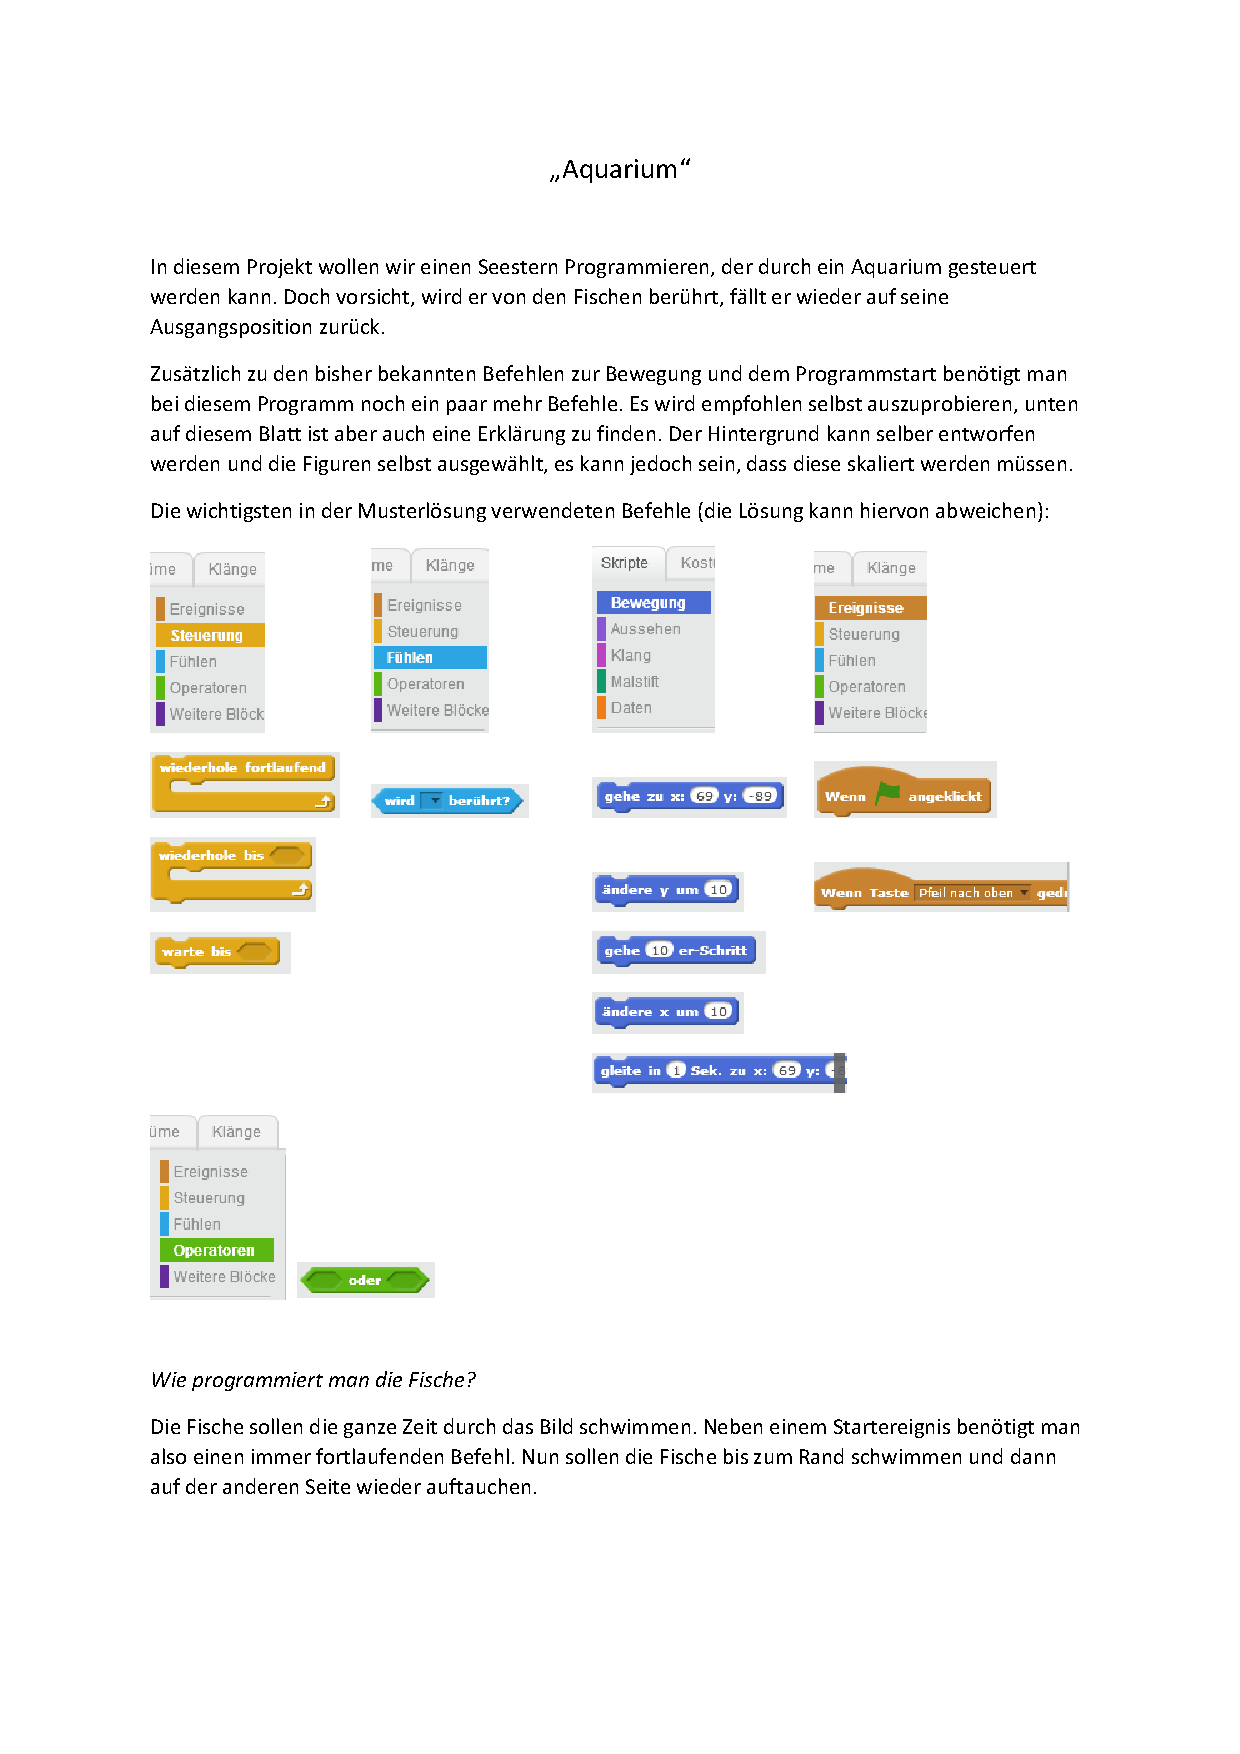
\includepdf[pages=-]{Anhang/ArbeitsblattAquarium.pdf}
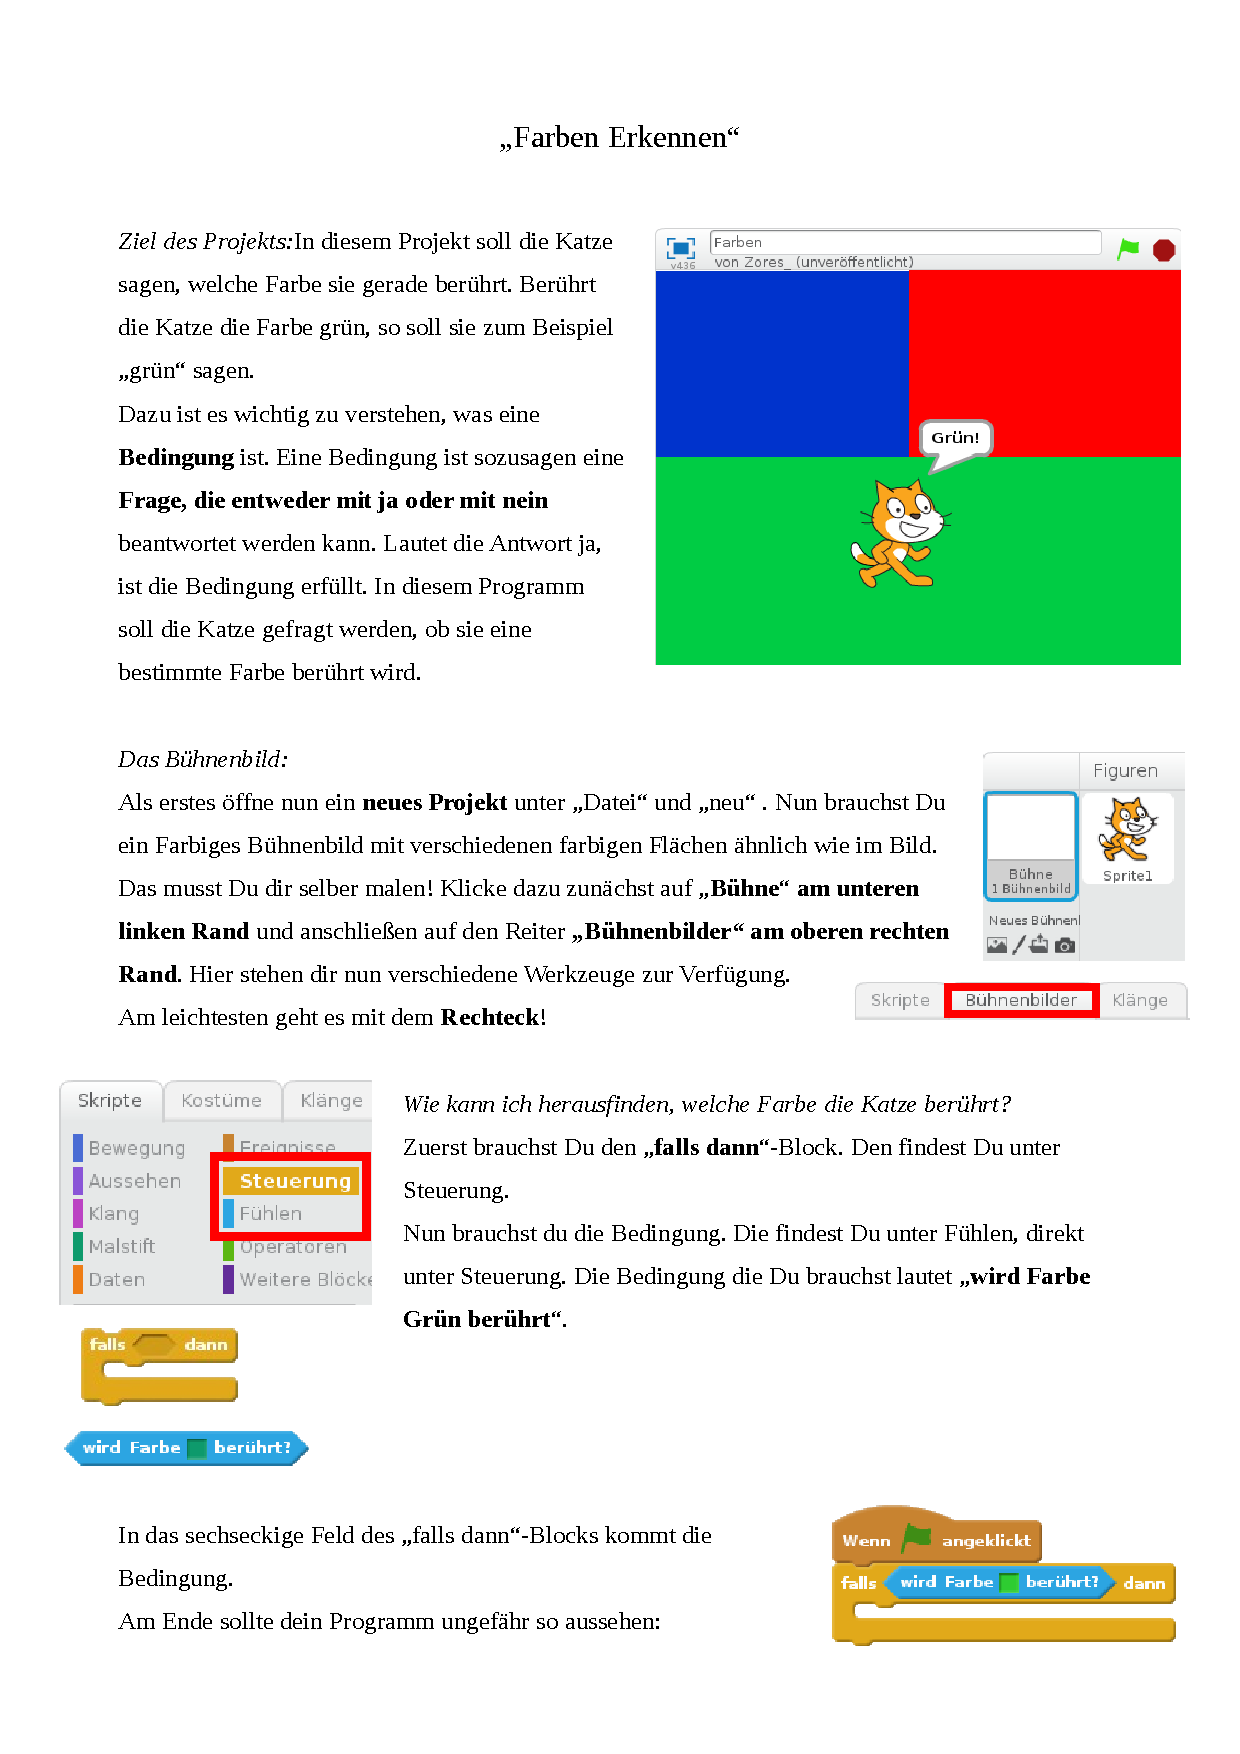
\includepdf[pages=-]{Anhang/ArbeitsblattFarbenerkennen.pdf}
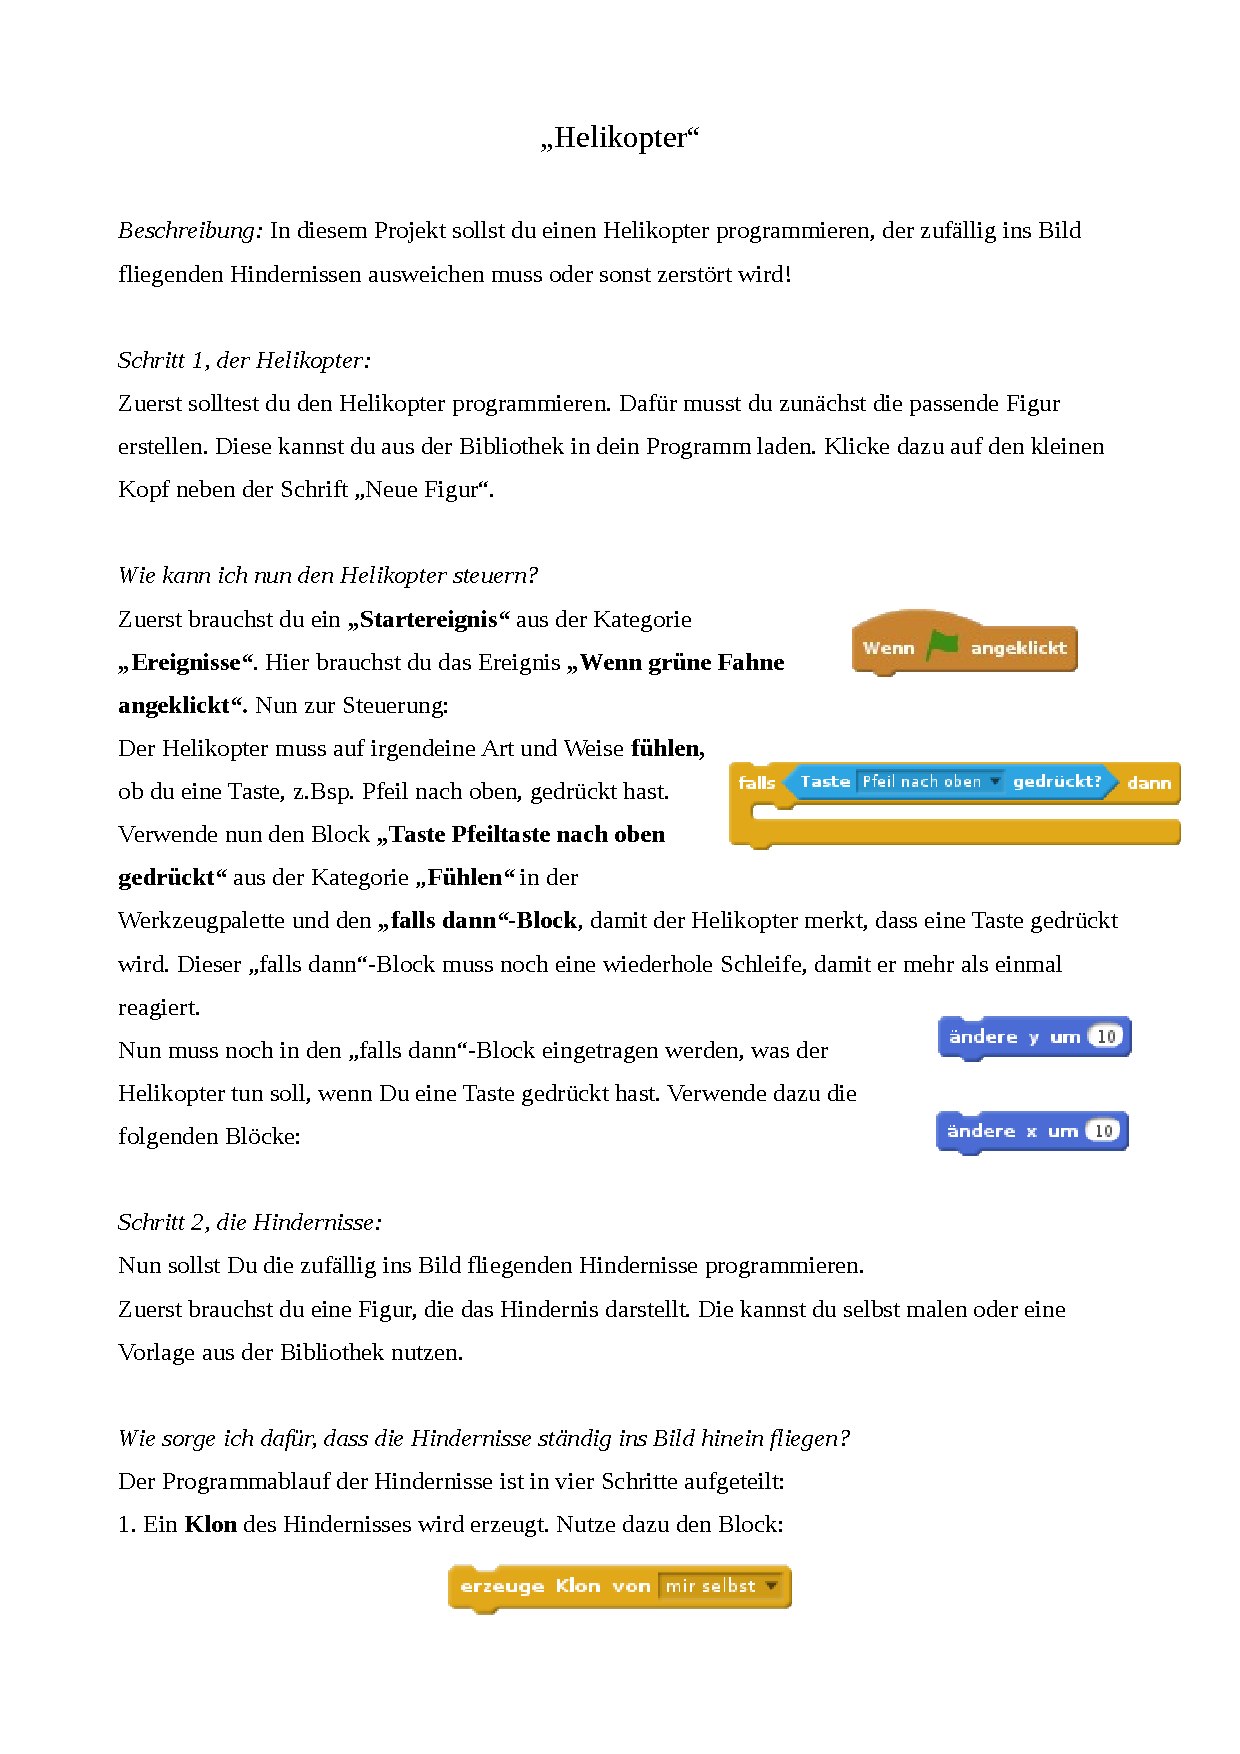
\includepdf[pages=-]{Anhang/ArbeitsblattHelikopter.pdf}
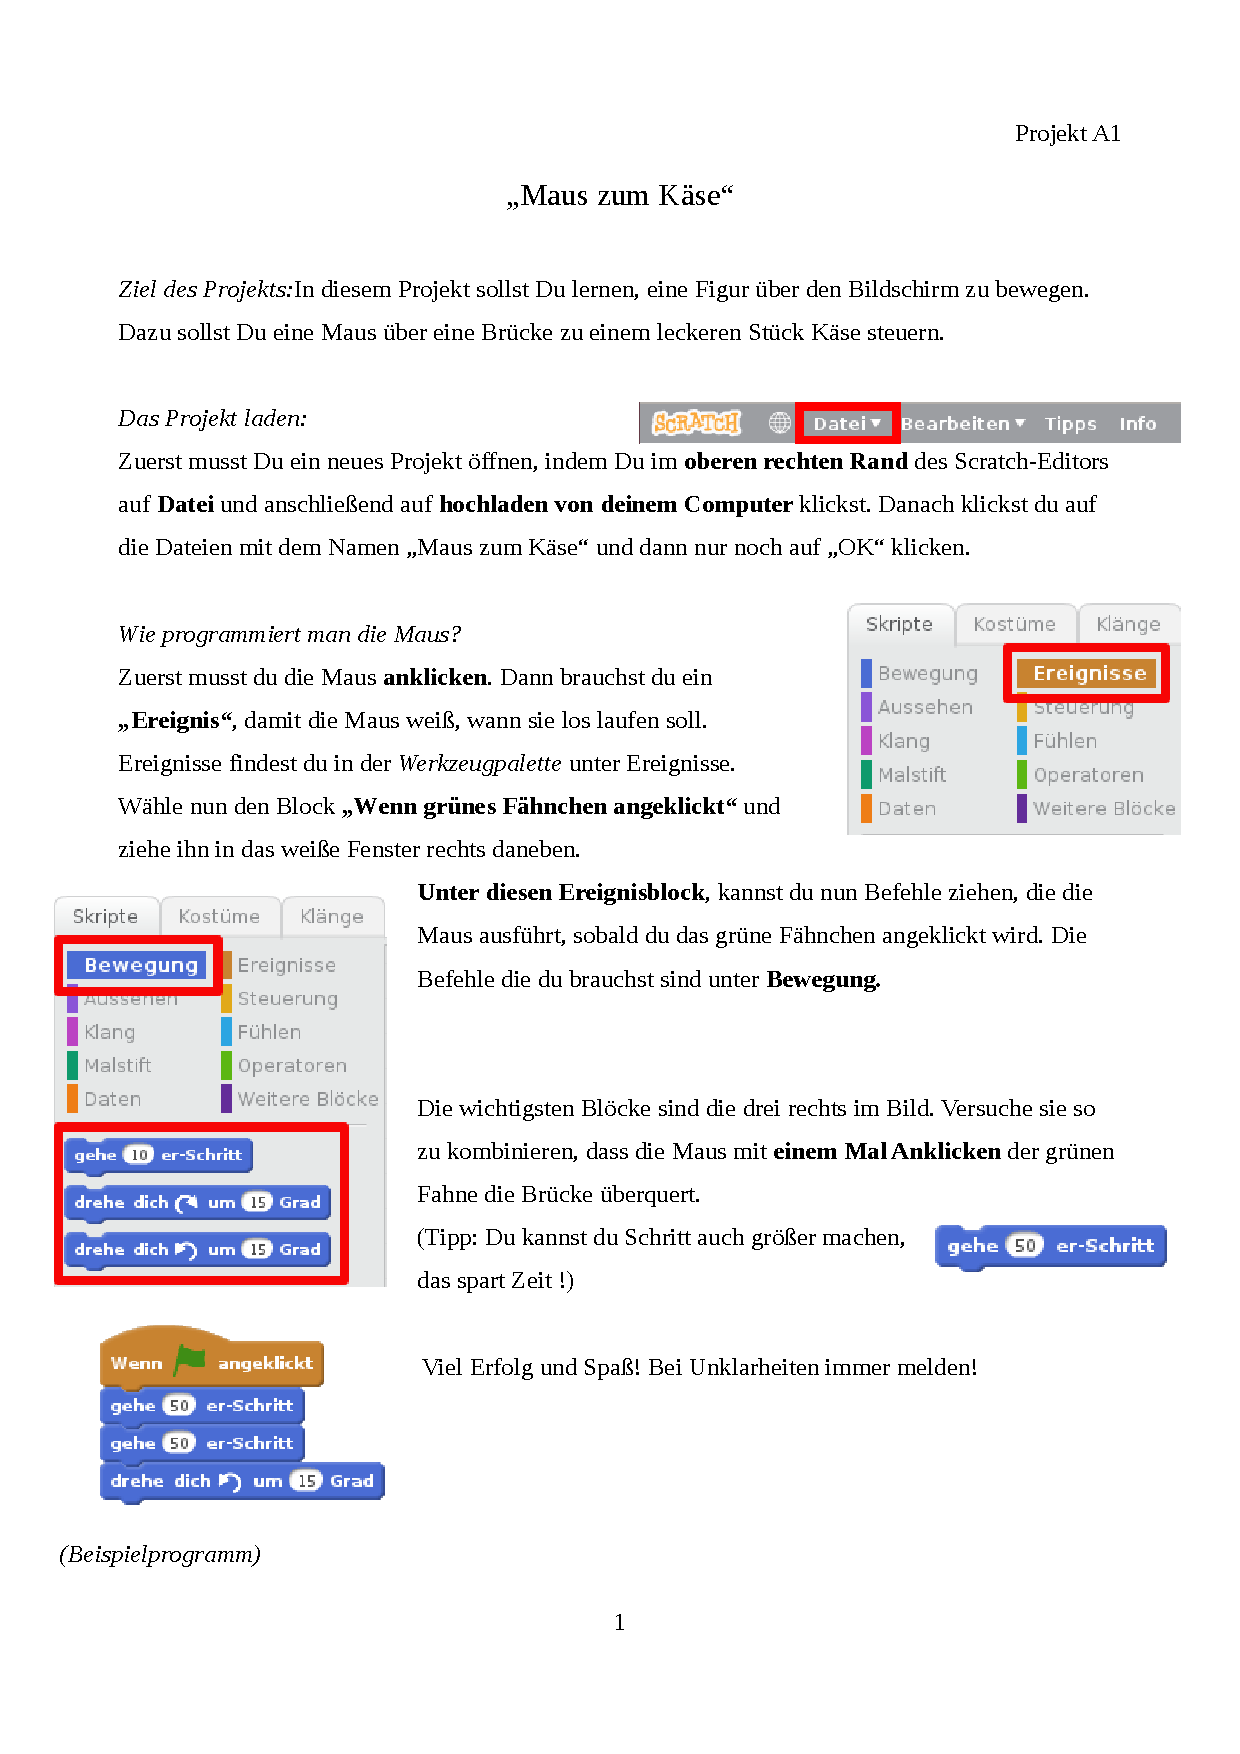
\includepdf[pages=-]{Anhang/ArbeitsblattMauszumKaese.pdf}
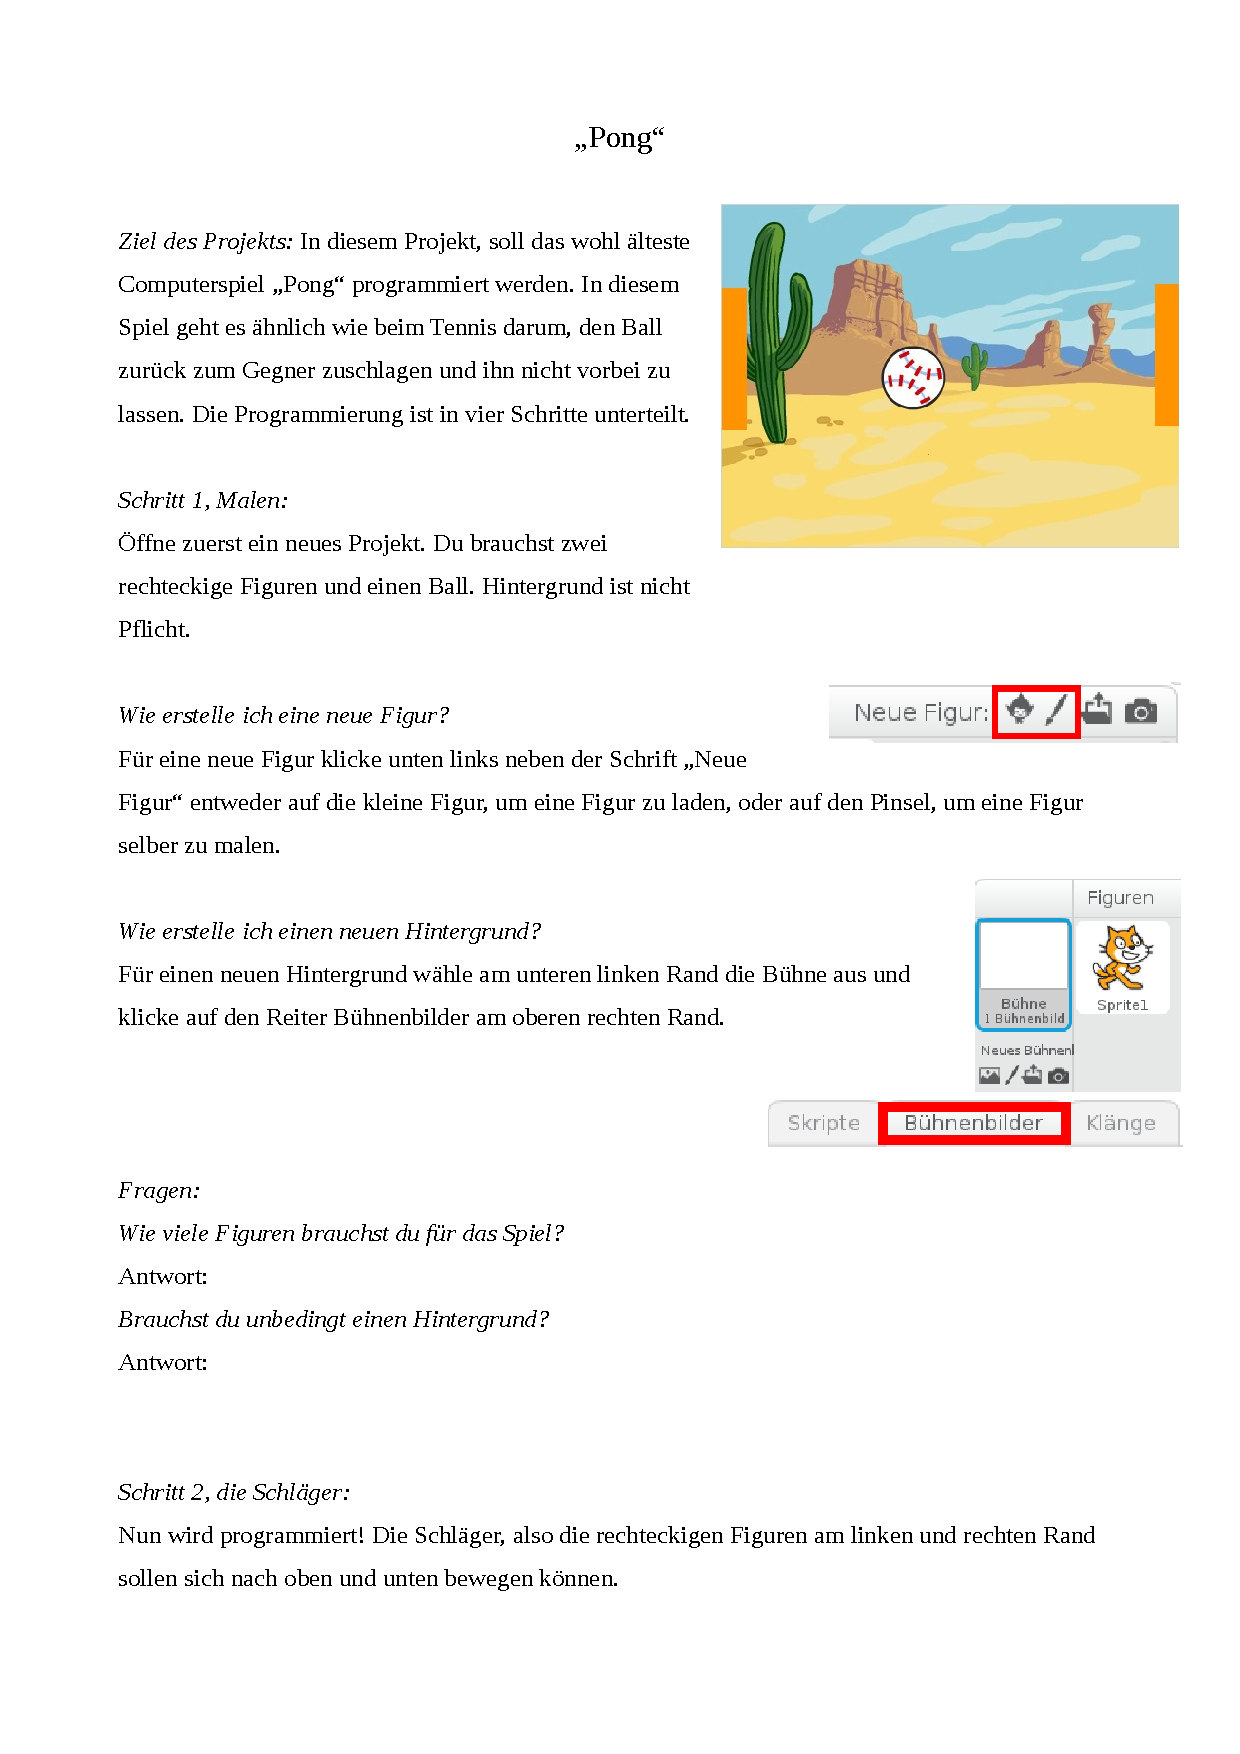
\includepdf[pages=-]{Anhang/ArbeitsblattPong.pdf}


%\section{Creative Commons Attribution-ShareAlike 4.0 International Public License}

By exercising the Licensed Rights (defined below), You accept and agree to be bound by the terms and conditions of this Creative Commons Attribution-ShareAlike 4.0 International Public License ("Public License"). To the extent this Public License may be interpreted as a contract, You are granted the Licensed Rights in consideration of Your acceptance of these terms and conditions, and the Licensor grants You such rights in consideration of benefits the Licensor receives from making the Licensed Material available under these terms and conditions.

Section 1 – Definitions.

    
\begin{itemize}
\item Adapted Material means material subject to Copyright and Similar Rights that is derived from or based upon the Licensed Material and in which the Licensed Material is translated, altered, arranged, transformed, or otherwise modified in a manner requiring permission under the Copyright and Similar Rights held by the Licensor. For purposes of this Public License, where the Licensed Material is a musical work, performance, or sound recording, Adapted Material is always produced where the Licensed Material is synched in timed relation with a moving image.
\item Adapter's License means the license You apply to Your Copyright and Similar Rights in Your contributions to Adapted Material in accordance with the terms and conditions of this Public License.
\item BY-SA Compatible License means a license listed at creativecommons.org/compatiblelicenses, approved by Creative Commons as essentially the equivalent of this Public License.
\item Copyright and Similar Rights means copyright and/or similar rights closely related to copyright including, without limitation, performance, broadcast, sound recording, and Sui Generis Database Rights, without regard to how the rights are labeled or categorized. For purposes of this Public License, the rights specified in Section 2(b)(1)-(2) are not Copyright and Similar Rights.
\item Effective Technological Measures means those measures that, in the absence of proper authority, may not be circumvented under laws fulfilling obligations under Article 11 of the WIPO Copyright Treaty adopted on December 20, 1996, and/or similar international agreements.
\item Exceptions and Limitations means fair use, fair dealing, and/or any other exception or limitation to Copyright and Similar Rights that applies to Your use of the Licensed Material.
\item License Elements means the license attributes listed in the name of a Creative Commons Public License. The License Elements of this Public License are Attribution and ShareAlike.
\item Licensed Material means the artistic or literary work, database, or other material to which the Licensor applied this Public License.
\item Licensed Rights means the rights granted to You subject to the terms and conditions of this Public License, which are limited to all Copyright and Similar Rights that apply to Your use of the Licensed Material and that the Licensor has authority to license.
\item Licensor means the individual(s) or entity(ies) granting rights under this Public License.
\item Share means to provide material to the public by any means or process that requires permission under the Licensed Rights, such as reproduction, public display, public performance, distribution, dissemination, communication, or importation, and to make material available to the public including in ways that members of the public may access the material from a place and at a time individually chosen by them.
\item Sui Generis Database Rights means rights other than copyright resulting from Directive 96/9/EC of the European Parliament and of the Council of 11 March 1996 on the legal protection of databases, as amended and/or succeeded, as well as other essentially equivalent rights anywhere in the world.
\item You means the individual or entity exercising the Licensed Rights under this Public License. Your has a corresponding meaning.
\end{itemize}


Section 2 – Scope.

    License grant.
        Subject to the terms and conditions of this Public License, the Licensor hereby grants You a worldwide, royalty-free, non-sublicensable, non-exclusive, irrevocable license to exercise the Licensed Rights in the Licensed Material to:
            reproduce and Share the Licensed Material, in whole or in part; and
            produce, reproduce, and Share Adapted Material.
        Exceptions and Limitations. For the avoidance of doubt, where Exceptions and Limitations apply to Your use, this Public License does not apply, and You do not need to comply with its terms and conditions.
        Term. The term of this Public License is specified in Section 6(a).
        Media and formats; technical modifications allowed. The Licensor authorizes You to exercise the Licensed Rights in all media and formats whether now known or hereafter created, and to make technical modifications necessary to do so. The Licensor waives and/or agrees not to assert any right or authority to forbid You from making technical modifications necessary to exercise the Licensed Rights, including technical modifications necessary to circumvent Effective Technological Measures. For purposes of this Public License, simply making modifications authorized by this Section 2(a)(4) never produces Adapted Material.
        Downstream recipients.
            Offer from the Licensor – Licensed Material. Every recipient of the Licensed Material automatically receives an offer from the Licensor to exercise the Licensed Rights under the terms and conditions of this Public License.
            Additional offer from the Licensor – Adapted Material. Every recipient of Adapted Material from You automatically receives an offer from the Licensor to exercise the Licensed Rights in the Adapted Material under the conditions of the Adapter’s License You apply.
            No downstream restrictions. You may not offer or impose any additional or different terms or conditions on, or apply any Effective Technological Measures to, the Licensed Material if doing so restricts exercise of the Licensed Rights by any recipient of the Licensed Material.
        No endorsement. Nothing in this Public License constitutes or may be construed as permission to assert or imply that You are, or that Your use of the Licensed Material is, connected with, or sponsored, endorsed, or granted official status by, the Licensor or others designated to receive attribution as provided in Section 3(a)(1)(A)(i).

    Other rights.
        Moral rights, such as the right of integrity, are not licensed under this Public License, nor are publicity, privacy, and/or other similar personality rights; however, to the extent possible, the Licensor waives and/or agrees not to assert any such rights held by the Licensor to the limited extent necessary to allow You to exercise the Licensed Rights, but not otherwise.
        Patent and trademark rights are not licensed under this Public License.
        To the extent possible, the Licensor waives any right to collect royalties from You for the exercise of the Licensed Rights, whether directly or through a collecting society under any voluntary or waivable statutory or compulsory licensing scheme. In all other cases the Licensor expressly reserves any right to collect such royalties.

Section 3 – License Conditions.

Your exercise of the Licensed Rights is expressly made subject to the following conditions.

    Attribution.

        If You Share the Licensed Material (including in modified form), You must:
            retain the following if it is supplied by the Licensor with the Licensed Material:
                identification of the creator(s) of the Licensed Material and any others designated to receive attribution, in any reasonable manner requested by the Licensor (including by pseudonym if designated);
                a copyright notice;
                a notice that refers to this Public License;
                a notice that refers to the disclaimer of warranties;
                a URI or hyperlink to the Licensed Material to the extent reasonably practicable;
            indicate if You modified the Licensed Material and retain an indication of any previous modifications; and
            indicate the Licensed Material is licensed under this Public License, and include the text of, or the URI or hyperlink to, this Public License.
        You may satisfy the conditions in Section 3(a)(1) in any reasonable manner based on the medium, means, and context in which You Share the Licensed Material. For example, it may be reasonable to satisfy the conditions by providing a URI or hyperlink to a resource that includes the required information.
        If requested by the Licensor, You must remove any of the information required by Section 3(a)(1)(A) to the extent reasonably practicable.
    ShareAlike.

    In addition to the conditions in Section 3(a), if You Share Adapted Material You produce, the following conditions also apply.
        The Adapter’s License You apply must be a Creative Commons license with the same License Elements, this version or later, or a BY-SA Compatible License.
        You must include the text of, or the URI or hyperlink to, the Adapter's License You apply. You may satisfy this condition in any reasonable manner based on the medium, means, and context in which You Share Adapted Material.
        You may not offer or impose any additional or different terms or conditions on, or apply any Effective Technological Measures to, Adapted Material that restrict exercise of the rights granted under the Adapter's License You apply.

Section 4 – Sui Generis Database Rights.

Where the Licensed Rights include Sui Generis Database Rights that apply to Your use of the Licensed Material:

    for the avoidance of doubt, Section 2(a)(1) grants You the right to extract, reuse, reproduce, and Share all or a substantial portion of the contents of the database;
    if You include all or a substantial portion of the database contents in a database in which You have Sui Generis Database Rights, then the database in which You have Sui Generis Database Rights (but not its individual contents) is Adapted Material, including for purposes of Section 3(b); and
    You must comply with the conditions in Section 3(a) if You Share all or a substantial portion of the contents of the database.

For the avoidance of doubt, this Section 4 supplements and does not replace Your obligations under this Public License where the Licensed Rights include other Copyright and Similar Rights.

Section 5 – Disclaimer of Warranties and Limitation of Liability.

    Unless otherwise separately undertaken by the Licensor, to the extent possible, the Licensor offers the Licensed Material as-is and as-available, and makes no representations or warranties of any kind concerning the Licensed Material, whether express, implied, statutory, or other. This includes, without limitation, warranties of title, merchantability, fitness for a particular purpose, non-infringement, absence of latent or other defects, accuracy, or the presence or absence of errors, whether or not known or discoverable. Where disclaimers of warranties are not allowed in full or in part, this disclaimer may not apply to You.
    To the extent possible, in no event will the Licensor be liable to You on any legal theory (including, without limitation, negligence) or otherwise for any direct, special, indirect, incidental, consequential, punitive, exemplary, or other losses, costs, expenses, or damages arising out of this Public License or use of the Licensed Material, even if the Licensor has been advised of the possibility of such losses, costs, expenses, or damages. Where a limitation of liability is not allowed in full or in part, this limitation may not apply to You.

    The disclaimer of warranties and limitation of liability provided above shall be interpreted in a manner that, to the extent possible, most closely approximates an absolute disclaimer and waiver of all liability.

Section 6 – Term and Termination.

    This Public License applies for the term of the Copyright and Similar Rights licensed here. However, if You fail to comply with this Public License, then Your rights under this Public License terminate automatically.

    Where Your right to use the Licensed Material has terminated under Section 6(a), it reinstates:
        automatically as of the date the violation is cured, provided it is cured within 30 days of Your discovery of the violation; or
        upon express reinstatement by the Licensor.
    For the avoidance of doubt, this Section 6(b) does not affect any right the Licensor may have to seek remedies for Your violations of this Public License.
    For the avoidance of doubt, the Licensor may also offer the Licensed Material under separate terms or conditions or stop distributing the Licensed Material at any time; however, doing so will not terminate this Public License.
    Sections 1, 5, 6, 7, and 8 survive termination of this Public License.

Section 7 – Other Terms and Conditions.

    The Licensor shall not be bound by any additional or different terms or conditions communicated by You unless expressly agreed.
    Any arrangements, understandings, or agreements regarding the Licensed Material not stated herein are separate from and independent of the terms and conditions of this Public License.

Section 8 – Interpretation.

    For the avoidance of doubt, this Public License does not, and shall not be interpreted to, reduce, limit, restrict, or impose conditions on any use of the Licensed Material that could lawfully be made without permission under this Public License.
    To the extent possible, if any provision of this Public License is deemed unenforceable, it shall be automatically reformed to the minimum extent necessary to make it enforceable. If the provision cannot be reformed, it shall be severed from this Public License without affecting the enforceability of the remaining terms and conditions.
    No term or condition of this Public License will be waived and no failure to comply consented to unless expressly agreed to by the Licensor.
    Nothing in this Public License constitutes or may be interpreted as a limitation upon, or waiver of, any privileges and immunities that apply to the Licensor or You, including from the legal processes of any jurisdiction or authority.


\end{document}
